\documentclass[12pt,oneside]{report}
\usepackage{amssymb,amsmath,amsthm,OU-Dissertation}
\usepackage{algorithm}
\usepackage{algorithmic}
\usepackage{rotating}
\usepackage[printonlyused,withpage]{acronym}
\usepackage{color}
\usepackage{enumitem}
\usepackage[english]{babel}
\usepackage{blindtext}

% Use one or the other.
\usepackage{natbib}
%\usepackage{cite}

%\usepackage{hyperref}
\usepackage
[
pdftex,
bookmarks,
pdftitle={Sensitivity Analysis of Code Carrier Coherence in the GPS Satellite
Fleet to Reduce Overbounding in WAAS to Increase Availability While Maintaining Integrity},
pdfauthor={Chad S. Sherrell},
pdfsubject={University of Oklahoma Ph.D. Dissertation},
pdfkeywords={Chad, Sherrell, Dissertation, WAAS},
hypertexnames=false,
colorlinks=true,
linkcolor=blue,
citecolor=blue,
urlcolor=blue
]
{hyperref}

\usepackage[procnames]{listings}

\providecommand{\tightlist}{%
  \setlength{\itemsep}{0pt}\setlength{\parskip}{0pt}}

%\usepackage{multirow}
%\usepackage{subfigure}
%\usepackage{graphicx}

%\ifx\pdfoutput\undefined
%\usepackage{graphicx}
%\else
%\usepackage[pdftex]{graphicx}
%\fi

%\onehalfspacing    % one & half spaced texts
%\singlespacequote  % single spaced quotes

%If the dissertation has a chapter that consists
%of 10 or more sections, a section that consists
%of 10 or more subsections, etc., uncomment the
% following line:
% \longtocentry

%%%%%%%%%%%%%%%%%%%%%%%%%%%%%%%%%%%%%%%%%%%%%%%%%%%%%%%%%%%%%%%%%%%%%%%%%%%%%%%

% TITLE
\title{Sensitivity Analysis of Code Carrier Coherence in the GPS Satellite
Fleet to Reduce Overbounding in WAAS to Increase Availability While Maintaining
Integrity}

%%%%%%%%%%%%%%%%%%%%%%%%%%%%%%%%%%%%%%%%%%%%%%%%%%%%%%%%%%%%%%%%%%%%%%%%%%%%%%%

%% SUPERVISORS
%%% One Supervisor
%\supervisor{James J. Sluss, Jr.}

%% Two Supervisors
\supervisor[James J. Sluss, Jr.]
{John W. Dyer}

%%% Three Supervisors
%\supervisor[James J. Sluss, Jr.]
%[John W. Dyer]
%{John E. Fagan}

%%%%%%%%%%%%%%%%%%%%%%%%%%%%%%%%%%%%%%%%%%%%%%%%%%%%%%%%%%%%%%%%%%%%%%%%%%%%%%%

\committeesize{5}

% FULL NAME; Combination of Upper/Lowercases
\author{Chad S. Sherrell}

% Default is B.S., M.S. If you have previous degree(s)
% other than them, uncomment the following line
% and enter your degree name(s).
%\previousdegrees{B.S.}

% The default is `Doctor of Philosophy' and `Ph.\ D.'
% If your target degree is other than the above,
% uncomment the following and enter your degree name.
%\degree{Master of Science}
%\degreeabbr{M.S.}

%% Can seem to make this work. -CSS
%\address{2311 North Los Robles Avenue}
%\\
%Apt 4A\\
%Pasadena, California\ \ 91104\\
%U.S.A.}

%\doctype{thesis}   % dissertation or thesis
                    % Dissertation is the default.
%\typeist{Mary K. Peterson} % if someone else typesets
                            % Author's name is the default.

% The system reasonably guesses the graduation
% year and month by looking at the system clock.
% The graduation month is either May, August, or December.
\graduationmonth{December} % Either May, August, or December
\graduationyear{2018} % 4 digit, not 2 digit

% \makeatletter
% \newcommand{\acx}{\protect\@acx}%
% \newcommand{\@acx}[1]{%
  % \ifAC@dua
   % \acl{#1}%
  % \else
   % \expandafter\ifx\csname ac@#1\endcsname\AC@used
      % \acs{#1}%
   % \else
      % \acl{#1}%
   % \fi
  % \fi
% }
% \makeatother

\begin{document}

\definecolor{keywords}{RGB}{255,0,90}
\definecolor{comments}{RGB}{0,0,113}
\definecolor{red}{RGB}{160,0,0}
\definecolor{green}{RGB}{0,150,0}
\definecolor{blue}{RGB}{0,0,255}

\setlength{\unitlength}{1.00 in}

% Title Page - Required
\titlepage

% Signature Page - Required
\signaturepage

% Copyright Page - Required
\copyrightpage

% Dedication - Optional
% No page numbering.
\newpage
%\mbox{\ }
%\newpage
\begin{dedication}
To my grandma, Joy Lee Green, who never gave up on me and never allowed me give up.
\end{dedication}

\thispagestyle{empty}

% Reset page number to 4 in case there was a Dedication section should not have page
% Numbering
\setcounter{page}{4}

%\newpage
%\thispagestyle{empty}
%\mbox{\ }

% Acknowledgements - Optional
\newpage
\acknowledgements     % NOT: \begin{ack...} ... \end{ack...}
\paragraph{Eric Altshuler}~\\
Technical consultation.

\paragraph{Emily McCord}~\\
Prototype runs.


% Table of Contents - Required
\tableofcontents

% List of Tables
% Required if you have tables
\listoftables

% List of Figures
% Required if you have figures
\listoffigures

\acronyms
\begin{acronym}[WAAS]
\acro{amqp}[AMQP]{Advanced Message Queuing Protocol}
\acro{ascii}[ASCII]{American Standard Code for Information Interchange}
\acro{cat}[CAT]{Collection and Analysis Tools}
\acro{ccc}[CCC]{Code Carrier Coherence}
\acro{cots}[COTS]{Commercial Off-The-Shelf}
\acro{cpu}[CPU]{Central Processing Unit}
\acro{crc}[CRC]{Cyclic Redundancy Check}
\acro{dms}[DMS]{Data Management System}
\acro{ess}[ESS]{Enhanced Shadow System}
\acro{fe}[F\&E]{Facilities and Equipment}
\acro{faa}[FAA]{Federal Aviation Administration}
\acro{geo}[GEO]{Geostationary Earth Orbit}
\acro{gps}[GPS]{Global Positioning System}
\acro{gus}[GUS]{GEO Uplink Subsystem}
\acro{hdf}[HDF]{Hierarchical Data Format}
\acro{hmi}[HMI]{Hazardously Misleading Information}
\acro{hvac}[HVAC]{Heating, Ventilation, and Air Conditioning}
\acro{iaas}[IaaS]{Infrastructure as a Service}
\acro{ioc}[IOC]{Initial Operational Capability}
\acro{isa}[ISA]{Instruction Set Architecture}
\acro{mmac}[MMAC]{Mike Monroney Aeronautical Center}
\acro{nas}[NAS]{National Airway Systems}
\acro{nase}[NASE]{National Airway Systems Engineering}
%\acro{nase}[NASE]{\acl{nas} Engineering}
\acro{nets}[NETS]{National Engineering Test Structure}
\acro{nist}[NIST]{National Institute of Standards and Technology}
\acro{nfs}[NFS]{Network File System}
\acro{nocc}[NOCC]{National Operations Control Center}
\acro{oei}[OEI]{\ac{om} External Interface}
\acro{om}[O\&M]{Operations and Maintenance Station}
\acro{oltp}[OLTP]{On Line Transaction Processing}
\acro{olap}[OLAP]{On Line Analytical Processing}
\acro{osp}[OSP]{Operational System Parameter}
\acro{paas}[PaaS]{Platform as a Service}
\acro{pep}[PEP]{Program Execution Plan}
\acro{pocc}[POCC]{Pacific Operations Control Center}
\acro{rea}[REA]{Responsible Engineering Authority}
\acro{risc}[RISC]{Reduced Instruction Set Computing}
\acro{rpe2}[RPE2]{Relative Server Performance Estimate 2}
\acro{saas}[SaaS]{Software as a Service}
\acro{saves}[SAVES]{Strategic Sourcing for the Acquisition of Various Equipment and Supplies}
\acro{sis}[SIS]{Signal-in-Space}
\acro{sql}[SQL]{Structured Query Language}
\acro{sog}[SOG]{Satellite Operation Group}
\acro{sparc}[SPARC]{\textbf{S}calable \textbf{P}rocessor \textbf{ARCh}itecture}
\acro{ssm}[SSM]{System Support Modification}
\acro{tcs}[TCS]{Terrestrial Communications Subsystem}
\acro{ups}[UPS]{Uninterruptible Power Supply}
\acro{waas}[WAAS]{Wide-Area Augmentation System}
\acro{wms}[WMS]{Wide-Area Master Station}
\acro{wre}[WRE]{Wide-Area Reference Equipment}
\acro{wrs}[WRS]{Wide-Area Reference Station}
\acro{wsf}[WSF]{WAAS Support Facility}
\acro{wss}[WSS]{WAAS Support Services}
\end{acronym}


% Abstract - Optional
\abstract  % NOT: \begin{abstract} ... \end{abstract}
\blindmathtrue
\blindtext
%\blinditemize
%\blindtext
%\blindenumerate
%\blindtext
%\blinddescription

The \ac{waas} is enhanced and maintained by \ac{nase} at the \ac{faa}.

%\input text/NoCite

% The Text of the Dissertation - Required
% Introduction
\newpage
\thispagestyle{empty}
\acresetall
\chapter{Introduction}
\label{chapter:introduction}

This dissertation develops an extensive analysis tool for the \ac{waas} to show that the statistical overbounding of \ac{ccc}, an integrity measure of \ac{waas}, can be reduced to increase availability without reducing integrity. The \ac{waas} is a navigational aid developed by the \ac{faa} with the goal of providing improved accuracy, integrity and availability of the \ac{gps}, giving aviation users the ability to use \ac{gps} in all phases of flight.  \ac{waas} augments standard \ac{gps} by providing regional range correction values associated with satellite ranging errors in GPS due to the ionosphere, which is the most significant contributor to environmental \ac{gps} ranging error.  \ac{waas} also provides corrections for any detected system errors from the system itself.  Standard \ac{gps} allows a user receiver (with an inaccurate clock) to estimate its range to multiple in-view satellites and, with ephemeris information to determine each satellite's position, \ac{gps} can compute an estimate of the user position as shown in Figure~\ref{fig:GPS-Basic-Overview}.

\begin{figure}
	\centering
	\scalebox{.5}{
	\mbox{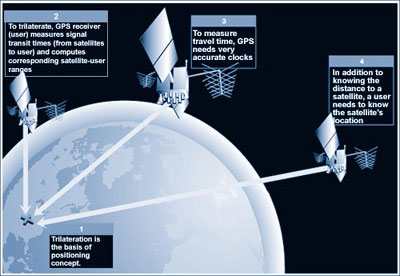
\includegraphics{figures/GPS-Basic-Overview.jpg}}
	}
	\caption{GPS Basic Overview. Trilateration is the basis of GPS positioning. A GPS receiver measures the signals transit times from satellites to the user and computes the corresponding satellite-user ranges. To measure travel time GPS needs a very accurate clocks. In addition to knowing the distance to the satellite, a user needs to know the satellites location.
  }
	\label{fig:GPS-Basic-Overview}
\end{figure}

\begin{figure}
	\centering
	\scalebox{.5}{
	\mbox{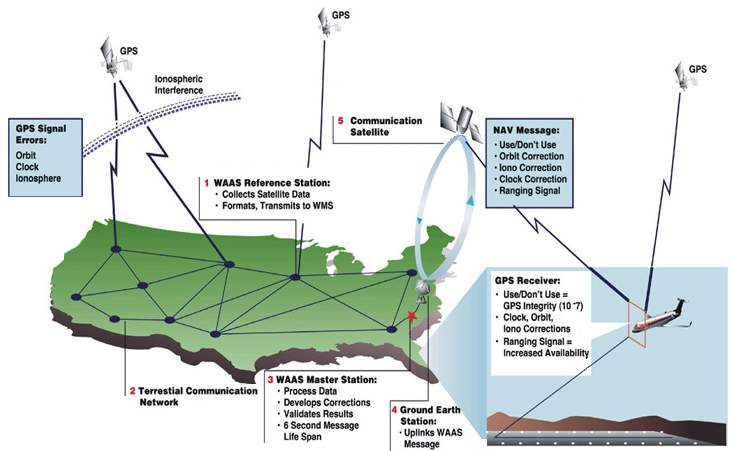
\includegraphics{figures/How-WAAS-Works.jpg}}
	}
	\caption{WAAS Basic Overview. The \acp{wrs} receive GPS measurements and transfer the data to the \ac{wms}. Integrity and differential corrections are generated and sent to the \ac{gus}.  The \ac{gus} transmits the \ac{wms} messages to a GEO Satellite which is broadcast down to users.
  }
	\label{fig:How-WAAS-Works}
\end{figure}

During normal operations, \ac{gps} \ac{sps} will have a user range error that is at or below a level required to support a positioning accuracy of 16 meters \ac{sep} \citep[p.51]{IS-GPS-200J}.  The \ac{waas} \ac{lpv} requirement specifies Horizontal Accuracy  of $\leq 1.5m$ error 95\% of the time Vertical Accuracy $\leq 2m$ error 95\% of the time \citep[p.4]{WAAS-PAN-66} \citep[p.34]{FAA-E-2892b}. \ac{waas} routinely meets this performance 99-100\% of the time \citep[p.29]{WAAS-PAN-66}. \ac{waas} estimates regional range correction values and provides these data to user receivers, which can incorporate the range corrections to improve the accuracy of the position solution, Figure~\ref{fig:How-WAAS-Works}. However, because the ranging errors are transmitted from a space-based component of the system, integrity checks must ensure that no false range corrections are transmitted that might cause significant erroneous position solutions.  There are a number of parameters in the \ac{waas} integrity checks that are statistically overbounded to ensure that no hazardous misleading information is transmitted to \ac{waas}-enabled \ac{gps} receivers.  Historically, the overbounding has been generous to provide significant safety tolerance \citep[p.61]{HMIDoc}, but no systematic study has been undertaken to identify which parameters are grossly overbounded and might possibly be reduced without affecting integrity.

The purpose of this sensitivity analysis is to isolate the performance of the \ac{ccc} integrity monitor and show the gains made to reduce its bounding variance so that an increase in availability is attained while integrity is maintained. The objective of the \ac{ccc} monitor is to detect satellite failures that cause the code phase and carrier phase of the \ac{gps} or \ac{geo} signal to be incoherent. Since the \ac{mops} user equipment uses carrier phase measurements to smooth the code phase (pseudorange) measurements, this is a potential source of user error. Further, the \ac{cnmp} monitor algorithm is based on the assumption that the code and carrier are coherent. Therefore, if the code and carrier are not coherent the multipath corrections can be in error and the \ac{udre} may not properly bound the user’s range error to that satellite.

The \ac{udre} and \ac{give} are the final values sent to the user which represent the accumulation of error bounding through the Integrity Data Monitors.  The \ac{ccc} calculation occurs towards the beginning of this flow and ensures the code and carrier are coherent before other monitors like \ac{cnmp} use the measurements. The final threshold selection for the \ac{udre} floor was based on the impact on system coverage as the \ac{udre} floor is increased. This run was done with 24 hours of data from December 20, 2000 using the prototype algorithm software. A floor of 4 (2.25 meters) was determine to be an optimal error bound based on this 24 hours run.

This dissertation is not intended to rationalize or disprove the setting of the \ac{udre} Floor bases on 24 hours of data analysis.  This sensitivity analysis is the initiation of a methodology to isolate the constituent elements that produce the final measurements composing the \ac{udre} and eventually the \ac{give}.  This detailed visibility into the system over a large data-set can be used to determine if the value has been set optimally or if further optimizations should be done base on empirical observations and there has never been an empirical analysis of its performance. Providing system integrity at all points and space at all times requires rigorous mathematical, statistical, and physical analysis. In fact it is estimated that to prove WAAS system integrity through observation alone would require nearly 50 years of data collection \citep[]{HOUSE-JUNE-2000}. This study is an interim step beyond the 24 hour data run, but less than 50 years of observations.  This rigorous study can be used to observe if a steady state he already occurred or can any trending be observed. The complexity of the system, and the volume of data to be analyzed to provide reliable sensitivity results has never been addressed in the literature.

% X If the code and carrier are assumed to be coherent, why do we need to monitor them?
% X Don't we monitor them precisely because we know they might not always be coherent?
% X I think this is better stated that the math requires the code and carrier to be coherent, so we monitor to ensure that this is the case.


% Make your first figure a basic GPS figure, then the WAAS system figure, then one that shows how corrections apply (see, for example, my Figure 2.7) Also, make your caption informative. It should have a title, then a description.  See any if my figures...
\begin{figure}
	\centering
	\scalebox{.35}{
	\mbox{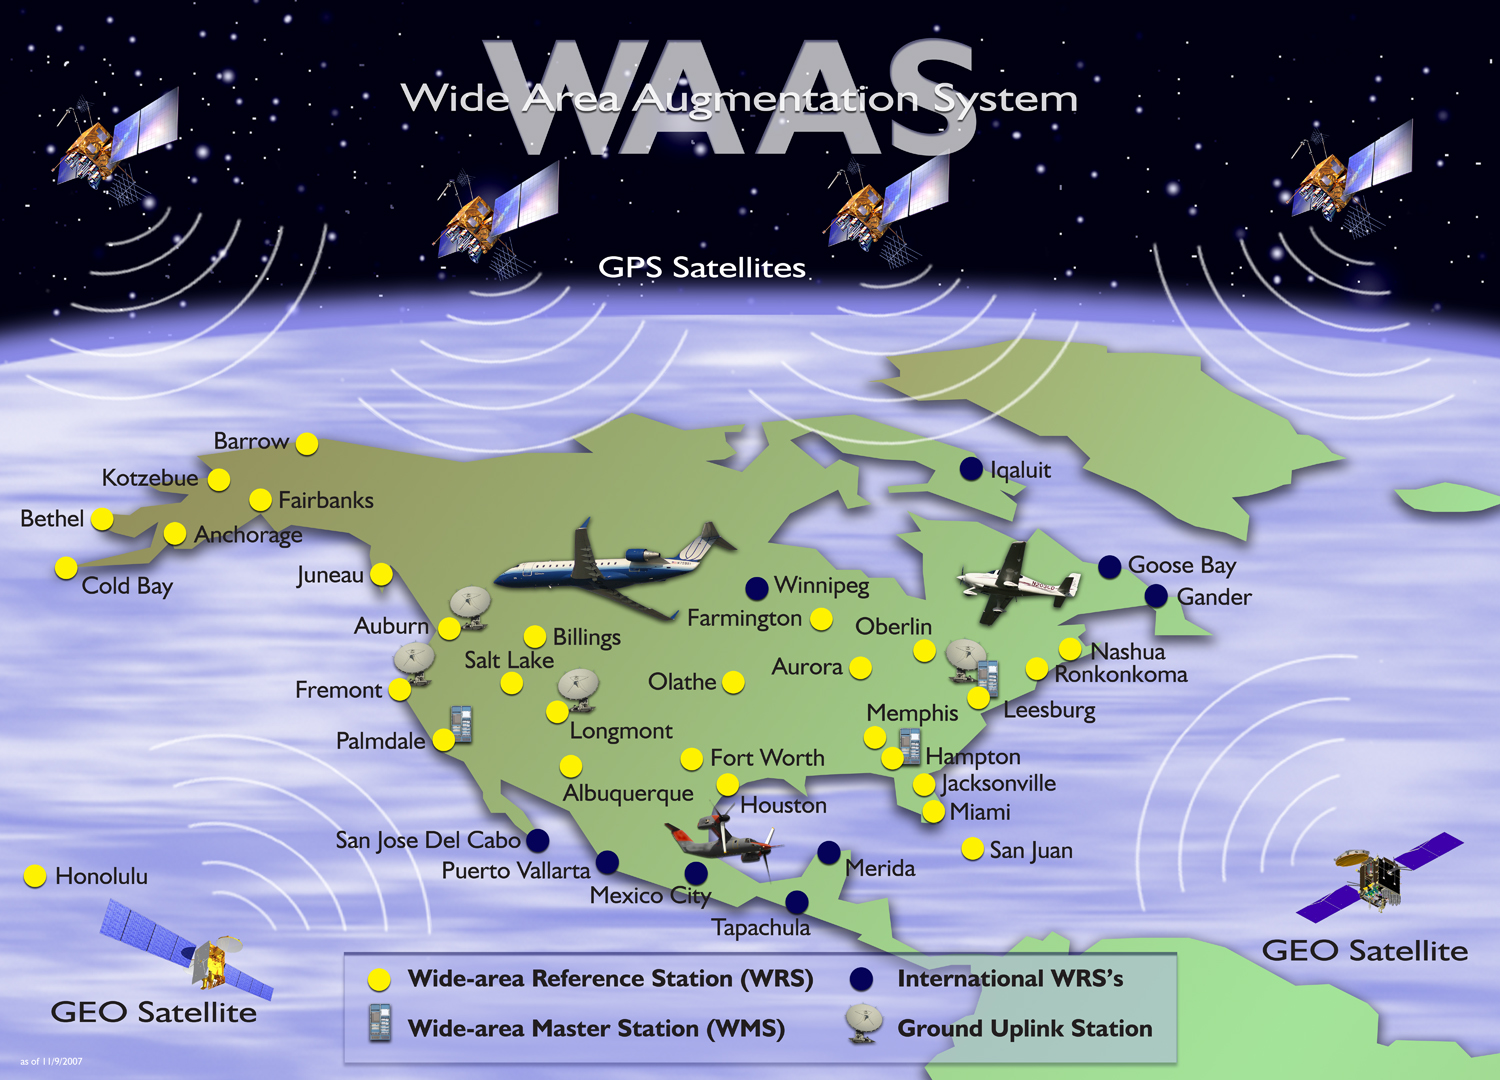
\includegraphics{figures/waas-overview-1.jpg}}
	}
	\caption{The Wide Area Augmentation System.  WAAS incorporates a number of reference stations in both the 48 contiguous United States as well as other North American partners: Mexico and Canada.  Three Master Stations calculate \ac{gps} satellite and ionospheric correction data and three GEO Satellites are use to transmit the information to aviation users.}
	\label{fig:WAAS-Overview-1}
\end{figure}

The stated goal of \ac{waas}, to provide improved accuracy, integrity and availability, is a complex set of tasks that may sometimes require tradeoffs between the competing goals.  The goals can be described as follows.  Accuracy is improved by providing a differential \ac{gps} solution, meaning \ac{waas} transmits range correction values for each satellite and the user \ac{gps} receiver applies these range correction values to the internally measured ranges prior to the user position computation.  This results in a \emph{differentially corrected} position solution that is more accurate than the position solution would be without the range corrections. The \ac{waas} architecture is a geographically diverse sensor network of high fidelity \ac{gps} receivers that track \ac{gps} satellites throughout North and Central America and Hawaii. This network consists of 114 \ac{gps} receivers at 38 geographically diverse sites.  Each \emph{reference station} is precisely surveyed at the antenna phase center, so the range to any in-view satellite is known (assuming accurate ephemeris information allows for accurate satellite position computation. The \ac{gps} receivers in the reference stations use receive-time (of the transmitted satellite signal) to estimate satellite range, so any error in local receiver time translates directly into an error in the range measurement to the \ac{gps} satellite. To provide the highest degree of accuracy the \ac{gps} antennas are designed to mitigate multipath and each \ac{gps} receiver clock is disciplined with a cesium frequency standard to provide a highly accurate and precise time source \citep[]{Kerkhoff}. A quarterly analysis of every second of every day is performed to observe if any change in the environment has occurred that may negatively affect performance. Yearly releases are conducted to update the antenna positions so that continental drift and other environmental factors are mitigated. The rigor put into this infrastructure enables this highly precise network of receivers to detect errors within \ac{gps} and the geographic diversity enables modeling of timing delays in the ionosphere. Once an end user within the \ac{waas} coverage area applies the \ac{gps} and ionospheric corrections sub-meter level \ac{gps} accuracy can be achieved in the best case and in the worst case range errors remain less than 2 meters. There are more than a dozen safety integrity monitors built into \ac{waas} that monitor \ac{gps} and ionospheric threats. Protecting users from integrity threats is an integral part of \ac{waas} as it was commissioned as a safety-of-life system, but integrity and availability have to be considered together as there is an inverse relationship between the two. As integrity increases availability is reduced. All \ac{gps} threats would be abated if \ac{gps} were not allowed to be used; integrity against \ac{gps} threats is 100\% while utilization of \ac{gps} is 0\%.  To achieve an acceptable level of utilization of \ac{gps} availability, confidence bounding is performed for \ac{gps} and ionospheric threats. The purpose of this study is to isolate the performance of the \ac{ccc} integrity monitor and show the gains made to reduce its bounding variance so that an increase in availability is attained while integrity is maintained. %You should note here that the trade off between availability and integrity is not strictly linear between 0 and 100.  You can increase availability from 0 to 95, and only reduce integrity in the nth decimal place.  10^-7, or something, right?, and use a REFERENCE!!!!!!!!

\ac{waas} has $\approx$2000 \ac{osp} values that define minimum and maximum limits, action thresholds, and timeouts [REF]. The parameters are used to control logic throughout the \ac{waas} system. There is always a balance between usability and safety.  For the \ac{faa} these two aspects are couched in the terms availability/continuity for usability and integrity for safety.  If the system remains off then this is the highest level of integrity, meaning if the user does not use the \ac{gps} then they are safe against all \ac{gps} related threats.  This would not make a practical system, so it led the engineers developing the \ac{waas} application to use values that would allow the system to be usable, but were significantly conservative to protect the user against \ac{gps} related threats.  At the inception of \ac{waas} there was insufficient empirical data to appropriately set many of the integrity bounding limits.  The CNMP has been stated as being grossly overbounded\citep[p.61]{HMIDoc}.  The \ac{nase} organization has now accumulated over 8 years of data, but there is currently no analytical system in place to process this volume of data so that updated \ac{osp} values can be set.

A sensitivity analysis of the type proposed in this study is difficult due to the shear magnitude of data to be analyzed. In order to properly analyze the sensitivity of \ac{waas} to the level of statistical overbounding of the \ac{ccc} parameter, many years of data must be analyzed.  This ensures that seasonal effects, a broad selection of significant weather events, and any astronomic effects can be included in the analysis [REF about what external things might affect integrity].  However, the system requirements for just the hardware and software present a significant barrier to achievement. Not only is significant processing power required, but an effective data handling method must also be employed so that the results are discoverable from the plethora of numerical information generated.  %Can you find a CS reference about such a system and its complexity?

%The cost of establishing and maintaining a high fidelity \ac{gps} monitoring network is considerable. Establishing the infrastructure and algorithms for the \ac{ioc} of \ac{waas} cost the United States government over \$4 Billion and the yearly maintenance cost are approximately \$100 million per year. Costs of this level prohibit all but a few countries from establishing a monitoring system of this magnitude. Further attaining access to the data along with the infrastructure to store and analyze the data is cost prohibitive. Over my tenure at the \ac{faa} there has been a concerted effort to establish the capability to perform an analysis of this extent. The infrastructure for collecting, storing and analyzing data at this volume has cost over \$5 million to establish and has pushed the limits of hardware and software.

The cost of establishing and maintaining the infrastructure for \ac{waas} is significant.  In addition to the 3 geosynchronous satellites keeping station above North America, there are the 38 reference station sites, three master reference stations, and six uplink stations, as well as the infrastructure to record and analyze daily information for uplink to the satellites.  Indeed, $\approx$374,284,800 data points are generated every day for analysis.  A major obstacle to performing any sensitivity analysis of the various overbounding parameters lies in the sheer volume of data that must be processed.  It should be noted that in order to glean any meaningful results, extended periods of historical raw data must be processed to ensure that seasonal variations, weather events, and astronomical transients (solar flares, magnetic storms, etc) are included in the analysis.  This research incorporates a system that is novel in itself.  The system capable of the desired analysis has taken several years and significant funding to develop. The system approach in this study utilizes commodity hardware and open source databases, programming languages and analytics software, with the goal of processing seven (7) years of data to assess the sensitivity of \ac{waas} to the \ac{ccc} parameter.  However, the system has been designed with the concept of scalability at the forefront, so that it can be expanded to assess other system sensitivities in the future.

%Though there was considerable time, effort and funding in establishing the capability outlined in this study, the approach in this study utilizes commodity hardware and open source databases, programming languages and analytics software. Further this capability was established to analyze as very specific data set. For the range measurements alone there are $\approx$374,284,800 data points per day.  The equipment required to process this was scaled commensurately for the data that is collected each day times the 7 years of data collected. Over 950 billion data points for just a single type of measurement and several hundred data elements are stored. The approach utilized in this study can be scaled appropriately to the application domain so cost for establishing a similar capability is tenable.

The approach outlined in this analysis is innovative in that it can be utilized to increase the availability of any Space Based Augmentation System while maintaining integrity.  This infrastructure is limited to all but a few countries, but with the countries that are developing this capability, world wide space based augmentation can be attained. The application of this methodology could lead to the establishment of highly available space based navigational aids on a global level. Further. the generalized approach utilized to solve this big data analytics problems can be utilized in domains outside of this specific aviation application.

\section{Chapter 1 Notes and Snippets}

Global SBAS Picture

\href{https://www.gps.gov/policy/funding/2017/}{https://www.gps.gov/policy/funding/2017/}

\href{http://commdocs.house.gov/committees/Trans/hpw106-100.000/hpw106-100\_1.HTM}{http://commdocs.house.gov/committees/Trans/hpw106-100.000/hpw106-100\_1.HTM}

\href{https://www.gps.gov/technical/ps/2008-waas-performance-standard.pdf}{https://www.gps.gov/technical/ps/2008-waas-performance-standard.pdf}

Things I need.

PRN SVN Mapping for the last five years.
Assign to Hoang.


First sentence what this dissertation has achieved.
30,000ft view of \ac{waas} and the Problem. Pros and Cons of \ac{waas} and the specific area I am looking at.

Paragraph 1: What is the problem?

Not more than 3-4 sentences telling the reader what the problem is, in as simple English as possible

Paragraph 2: Why is the problem hard?

What has eluded us in solving it? What does the literature say about this problem? What are the obstacles/challenges? Why is it non-trivial?

Paragraph 3: What is your approach/result to solving this problem?

How come you solved it? Think of this as your “startling” or “sit up and take notice” claims that your dissertation will plan to prove/demonstrate

Paragraph 4: What is the consequence of your approach?

So, now that you’ve made me sit up and take notice, what is the impact? What does your approach/result enable?
~\\

%This paragraph belongs above...I attempted to put it where it seems to fit...%


%Don't need any of this next paragraph in the Intro%
%Currently in this research effort the beginnings of a system have been created that can be used as an analytics platform for getting the varying data formats and elements into a common format where meaningful analysis can be performed.  Every component in the system is purposely selected or designed to take data from its rawest form and process it into a format that can be utilized, manipulated and assessed. As of this writing the system can process NovAtel GUST, G-II and G-III \ac{gps} receiver binary log files. The software can identify receiver log messages, \ac{crc} check that the messages is valid and break each message type into its constituent elements for storing and further analysis. This has been fully demonstrated end to end on a \ac{geo} Satellite monitoring system in development. This system is currently monitoring one \ac{geo} satellite at one \ac{gus} site but will be expanded to four \ac{geo}s at 8 \ac{gus} sites in the near future. It process data from the \ac{waas} application receiver and a second receiver used for fault isolation. The system is logging $\approx$1213 data elements per second from only two message types and this number will grow as more message types are recorded to the database.

\noindent
\url{http://commdocs.house.gov/committees/Trans/hpw106-100.000/hpw106-100_1.HTM}
\citep[]{HOUSE-JUNE-2000}

Third and most significant, while we can observe that the system is now performing very well, providing system integrity at all points and space at all times requires rigorous mathematical, statistical, and physical analysis. Proving the required level of integrity through observation alone would require nearly 50 years of data collection. Clearly, this is not acceptable. Instead, observation of the signal and collection of data over the next 2 years will be used to support analytical proof of the integrity required for FAA certification.
A group of experts has been formed to establish this road map for certification. The WIPP has been meeting almost monthly since February and is making very good progress.
If I may say a word in defense of the FAA, which has been criticized for its management of software-intensive programs, in the case of WAAS I would like to urge the committee not to lose sight of the fact that the Wide Area Augmentation System is the first time in the 45-year history of the FAA that a new navigation and landing technology is being commissioned for the entire national air space system. It will replace ILS and VOR technology that dates to the late 1940s and actually predates the formation of the FAA as we know it today.
WAAS is part of a world-wide movement toward satellite navigation. Japan and the European Union are developing their versions of the same technology. Chile has installed test bed equipment in anticipation of a South American WAAS system. This transition to satellite navigation is necessary if we are to avoid gridlock in the skies in the 21st century while also increasing safety.

\noindent
GPS Error Sources

\noindent
\url{https://en.wikipedia.org/wiki/
Error_analysis_for_the_Global_Positioning_System}

\noindent
GPS Error Sources

\noindent
\url{https://www.e-education.psu.edu/geog160/node/1924}

\newpage

\newpage
\thispagestyle{empty}
\acresetall
\chapter{Background and Literature Review}
\label{ch:background}

\section{Introduction to the \ac{gps}}\label{introduction-to-gps}

The \ac{gps} is a remarkable system for finding one's location and its success is largely due to the modest needs of the average user. Standard \ac{gps} accuracy is approximately 15 meters\citep[]{GPS_FOR_DUMMIES} and this level of accuracy is quite satisfactory for many applications, including land navigation, which is the primary consumer application for \ac{gps}. However, when \ac{gps} accuracy is discussed it is generally in terms of horizontal accuracy.  Vertical accuracy is seldom mentioned in the discussion of accuracy and most \ac{gps} manufacturers do not publish the vertical accuracy specification.  Due to this, a rule-of-thumb has developed that suggests that the vertical accuracy is only half as good as the horizontal accuracy.  So, if Standard \ac{gps} is accurate to within 15 meters in the horizontal, then it is considered accurate to about 30 meters in the vertical, which is unacceptable for aircraft landings. This is why the \ac{waas} and the \ac{laas} are indispensable for a \ac{gls}.  Many different factors affect the precision of \ac{gps} which will be explored during this overview of \ac{gps}.

\ac{gps} is comprised of 24 well placed satellites. The satellites orbit the earth in 6 orbital planes that are at a 55$^o$ inclination with 4 satellites per plane such that at least 4 satellites will be above the horizon at any given moment. This allows users the ability to use the system 24 hours a day anywhere on the planet. These satellites are not geo-orbital, but are at a \ac{meo} and orbit the earth twice a sidereal day with a speed of 3.9km per second.  The basic principal of the \ac{gps} system is quite simple.  A satellite orbits the earth at about 12,600 miles shown in Figure~\ref{fig:GPS_Basics_1}. \ac{gps} works by determining the range from the \ac{gps} satellite to the user receiver. The satellite acts as a reference point with a known location.  With one \ac{gps} satellite the user knows that he is on the sphere from the \ac{gps} satellite to the receiver. The user can be located anywhere on the surface of the sphere created by the range of the satellite to the user receiver. How this range is known will be discussed later.

\begin{figure}
  \centering
	\scalebox{.9}{
	\mbox{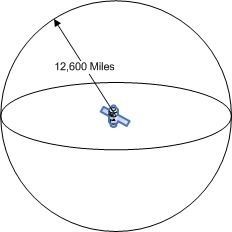
\includegraphics{figures/GPS_Basics_1.jpg}}
	}
  \caption{\ac{gps} Basics: Radius}
	\label{fig:GPS_Basics_1}
\end{figure}

Introducing another \ac{gps} satellite, the user can now be isolated to the intersection of two spheres which is a circle shown in Figure~\ref{fig:GPS_Basics_2}. When a third satellite is introduced it intersects the circle at two points shown in Figure~\ref{fig:GPS_Basics_3}. \ac{gps} assumes an earth centered, earth fixed, x-y-z 3D Cartesian coordinate system. Any location in this 3D space requires no more than 3 components to be completely identified. So, even though the intersection of 3 spheres yields two different points, the point located outside the earth's atmosphere is rendered useless by the earth centered earth fixed reference system. One point will be within Earth's atmosphere with an acceptable rate of velocity while the other
point will be in space traveling at a high velocity.

\begin{figure}
	\centering
	\scalebox{.5}{
	\mbox{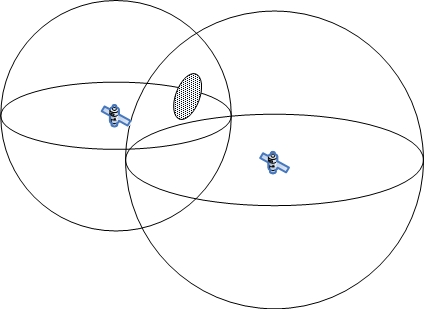
\includegraphics{figures/GPS_Basics_2.jpg}}
	}
	\caption{\ac{gps} Basics: Circle}
	\label{fig:GPS_Basics_2}
\end{figure}


\begin{figure}
	\centering
	\scalebox{.55}{
	\mbox{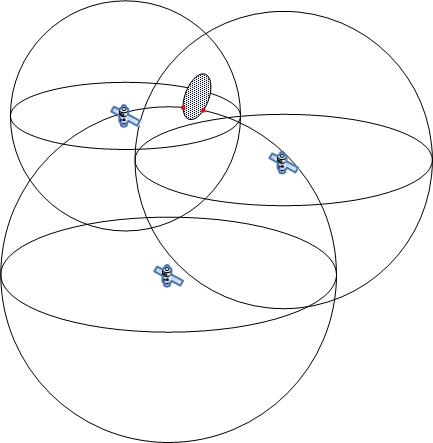
\includegraphics{figures/GPS_Basics_3.jpg}}
	}
	\caption{\ac{gps} Basics: Two Points}
	\label{fig:GPS_Basics_3}
\end{figure}

If the user measurements were perfect then three satellites would be
sufficient to determine the user's location, but to take near perfect
measurements would require the use of a highly stable atomic or optical
clock. These clocks are large, very expensive and require considerable
power, so the use of these types of clocks is impractical. Most \ac{gps}
receivers utilize a quartz crystal oscillator for timing. This
oscillator is small, cheap and low power but also very inaccurate, but,
as it turns out, if three measurement made with perfect time can be used to produce a position solution in 3-dimensional space then four imperfect measurements can be used to produce the same solution while solving for the receiver clock offset. \ac{gps} utilizes a fourth satellite to solve for the user's clock, synchronizing the receiver clock with \ac{gps} time. Since any clock offset from \ac{gps} universal time will affect all of the measurements, the receiver looks for a single correction factor that can be subtract from all its timing measurements that would cause them all to intersect at a single
point. When the clock offset is applied it brings the receiver's clock back into sync with \ac{gps} time. The fourth satellite helps calculate the timing correction and in turn a location correction and selects one of the remaining two points as the position. The fourth satellite allows for the solving of a
linear set of equations for x, y, z, and t simultaneously. Four satellites are required for (x,y,z,t) but in normal operation users are tracking more than four satellites; typically around 6 to 8. This sets up an overdetermined system of equations and a least-squares algorithm is used to determine the minimum error position solution. An added benefit is that every \ac{gps} receiver essentially has atomic-accuracy.

{[}Link: Getting Perfect Timing Using \ac{gps} for Timing{]}{[}3{]}\\
{[}Link: Trilateration algorithm for n amount of points{]}{[}4{]}

The satellites are used as reference points, but how can something moving high above the earth at a high velocity be used for measuring distance?  Every aspect of the \ac{gps} constellation is precisely monitored by six earth based monitor stations located throughout the world.  Any variance in the orbit, position, or velocity of a satellite is compensated and adjusted for at the master control station, located in Colorado Springs, Colorado.  These constant adjustments are put into a \ac{gps} message called the ephemeris message. The \textit{ephemeris} is a mathematical model of the motion of the orbit of a satellite. This model allows a \ac{gps} receiver to know the exact position of a satellite at a given time.  Now a method similar to \textit{trilateration} can be used to determine the \ac{gps} receiver's range or distance to the satellite. Trilateration uses the known locations of three or more reference points, and the measured distance between the subject and each reference point to determine the subject's location. In the case of \ac{gps} the distance is measured using the \ac{toa} of a ranging signal called the \textit{pseudorandom code}. The code is a very complex set of digital information that is called pseudorandom because it resembles random noise. It is repeated every millisecond. When the receiver receives the pseudorandom code it takes the signal propagation time multiplied by the speed of light to get the range to the satellite.  This is simple in concept, but the timing has to be near perfect.  If the time is off by even 1/1000 of a second the range could be off by 300,000 meters.  The \ac{gps} satellites actually keep track of their time using atomic clocks.  Each satellite is equipped with four atomic clocks to precisely track time, but atomic clocks are very costly and impractical for producing low cost \ac{gps} receivers.  Instead manufacturers use a less precise, less expensive crystal clock; but now have to overcome the error introduced by the receiver clock as previously mentioned.  Theses techniques allow users to track satellites, correct time and calculate ranges enabling one to find their position, but these ranges still contain errors; therefore they are referred to as \textit{pseudoranges}. \ac{gps} has many errors associated with it that cumulatively reduce \ac{gps} accuracy. Due to these errors the \ac{gps} signal does not meet the accuracy, integrity, availability, and
continuity requirements critical to safety of flight.  These errors can be accounted for using \ac{dgps} which is the method of using a \ac{gps} receiver at a fixed known reference point to determine the errors in \ac{gps} ranging.

\noindent
The errors can be categorized as follows:

\begin{itemize}
	\item Ephemeris ($<$ 1 meter Error)

The ephemeris is a mathematical model of the motion of the orbit of a satellite. This model is provided to the user and predicts where the satellite will be, but the forces acting upon the satellite don't always conform perfectly to the model. Any errors in the model will add to a user's position error, but since the ephemeris data is constantly being adjusted the error introduced is small and can be removed by differential \ac{gps} between two observations of short separation.

	\item Satellite Clock Errors ($<$ 1 meter Error)

Satellites use atomic clocks to precisely monitor time, but even atomic clocks are not perfect.  Since the pseudorange calculation is based on time any discrepancy in the clock will introduce error.  This can also be removed with differential \ac{gps}.

	\item Receiver Clock Errors (1 meter $<$ Error $<$ 2 meters)

A \ac{gps} Receiver uses a crystal clock which is much less accurate than an atomic clock; consequently additional timing errors exist.  The Receiver Clock produces more error than the Satellite Clock and unfortunately can not be removed with differential \ac{gps}, but is treated as another unknown during the estimation process.

	\item Ionosphere / Troposphere ($\approx$4 meters)

The atmosphere can be broken down into many layers but the two that most affect \ac{gps} are the ionosphere and the troposphere.  The \textit{ionoshpere} is the ionized part of Earth's upper atmosphereis and is a dispersive medium. The \ac{gps} signal incurs propagation delay as it is bent and changes speed when passing through the ionosphere. Though the delay is generally negligible, the ionosphere increases the speed of the carrier phase and slows down the pseudorandom code, so this source of error must be taken into consideration.  Temperature, pressure and humidity in the \textit{troposphere}, the lowest layer of the Earth's atmosphere, can also affect a \ac{gps} signal's propagation. The troposphere is a non dispersive medium, so the carrier phase and pseudorandom code are delayed by the same amount increasing the measured distance to the satellite from the actual distance.\cite[]{EL-RABBANY}.

 	\item \ac{gps} Satellite Geometry

A Satellite's geometry with respect to other satellites also plays a role in the position solution.  The closer the satellites are to one another the poorer the position solution and the more spread out the better the position solution.  The \ac{dop} is a number that represents the acceptability of the \ac{gps} geometry.  It can further be broken down into a horizontal and vertical component known as the \ac{hdop} and \ac{vdop}.

	\item Multipath

Multipath is a source of error that is introduced when the \ac{gps} signal is reflected from surfaces near the receiver's antenna, such as buildings, and the
reflections are mistaken for the primary signal. The reflected signal
adds additional propagation delay over the true signal, and in turn,
additional user error. This is the same occurrence that causes ghosting on a television set. \ac{waas} reduces the potential of this error source by using specialized \ac{gps} \acp{mla} and a priori siting analysis to avoid multipath generating structures.

	\item \ac{sa} ($>$ 10 Meters)

The last error that will be mentioned is artificial error.  The U.S. Military purposely skewed the \ac{gps} signal to artificially inflate the error in the system so that it could not be used against them.  When \ac{sa} was active it was the most substantial source of error, but the use of differential \ac{gps} could nearly eliminate \ac{sa}'s effectiveness. The use of \ac{sa} was discontinued on May 1, 2000.

\end{itemize}

\section{Differential \ac{gps} (DGPS)\label{section:DGPS}}

\ac{dgps} is the method of using a \ac{gps} receiver at a fixed known reference point to determine the errors in \ac{gps} ranging. To do this, the \ac{gps} receiver's antenna position is accurately surveyed.  Next, the difference is calculated between the pseudorange internally measured by the \ac{gps} receiver and the pseudorange calculated from a satellite's current \ac{gps} almanac, ephemeris information, and the surveyed location.  The difference between the measured pseudorange and the calculated pseudorange is the \textit{pseudorange correction} which is the distance that the local user should adjust a respective satellite's pseudorange by to achieve a minimum error position solution. The pseudorange correction is a lump sum adjustment for multiple sources of error which include ephemeris, satellite and receiver clocks, ionosphere and troposphere, and even Selective Availability. However, the pseudorange correction can only be computed by knowing the precise location of the reference receiver antenna. Another thing to note is that most \ac{dgps} systems make corrections in the range domain by adjusting the pseudorange measurement of each satellite in view.  An alternative approach is to adjust the system in the position domain.  This would involve calculating a position solution for the reference point then calculating a position correction vector.  This is generally not done due to the fact that position solutions are calculated by manufacturers using proprietary methods, and their behavior is not known a priori.

The many different \ac{dgps} solutions that have been developed fall broadly into two categories: post-processed and real time. Surveyors are a primary user of the non-real time post-processing category.  They collect \ac{gps} data from known reference points, which they call \textit{benchmarks}, and the point needing to be surveyed.  The distance between the benchmark and the survey point is called the \textit{baseline}, and it is generally preferred to use the benchmark with the shortest baseline to the survey point. After about 15 minutes to an hour of collecting data at both locations they can post process the data with \ac{gps} utilities to produce a position solution accurate to within a centimeter\footnote{Utilizes \ac{gps} L1/L2 survey equipment}.  On the other hand, real-time differential \ac{gps} systems acquire the data from the reference points, calculate the pseudorange corrections, and broadcast them out at a rate of 2 to 5 Hertz to be used in navigation applications. Since \ac{laas} falls into the real time category, it and a few other prominent real time \ac{dgps} systems will be discussed.

One of the first systems developed actually used the acronym \ac{dgps}, but sometimes also goes by \ac{ndgps} to distinguish \ac{dgps} the concept from \ac{dgps} the system.  The \ac{ndgps} is used by the U.S. Coast Guard in harbor regions to give ships better position solutions.  Even though the name implies national coverage is it limited to coastal regions. Europe and Canada also have similar solution for their heavily utilized maritime locations. There are even commercial companies like VERIPOS, StarFire, and OmniSTAR that provide \ac{dgps} services.

\begin{figure}
	\centering
	\scalebox{1.437}{
	\mbox{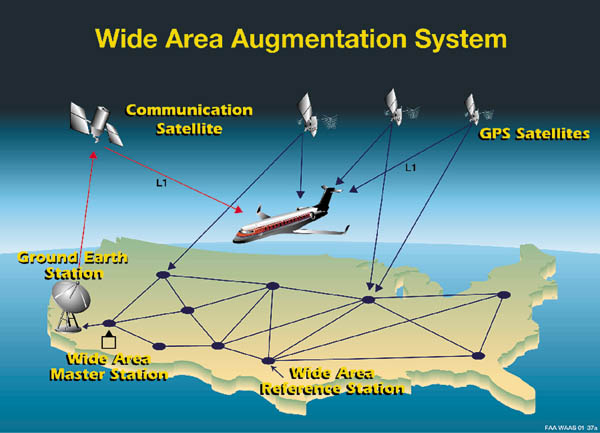
\includegraphics{figures/waas.jpg}}
	}
	\caption{Wide Area Augmentation System\citep[]{FAA_WAAS}}
	\label{fig:FAA_WAAS}
\end{figure}

Most of the \ac{dgps} systems developed had a very specific function or operated in such a localized area that it precluded widespread use. The \ac{faa} wanted to capitalize on the benefits of \ac{dgps} while promoting a broad coverage area. To that end they designed \ac{waas}, as shown in Figure~\ref{fig:FAA_WAAS}, established reference points throughout the contiguous United States. These fixed reference points were used to establish pseudorange corrections for most of North America.  \ac{waas} corrections are then sent to a geo-orbital satellite and broadcast to \ac{waas}-enabled \ac{gps} receivers.  \ac{waas} improved the accuracy of \ac{gps} to less than 2 meters in the horizontal and less than 3 meters in the vertical. This was a significant enhancement to \ac{gps}; an improved \ac{gps} position solution free for the end user.  \ac{gps} manufacturers adopted this readily and now \ac{waas}-enabled \ac{gps} receivers are commonplace. A major shortcoming with \ac{waas} is its confinement to North America.  Additional Reference Receivers are being installed in Alaska and Mexico, but this is still a United States / North America locale. Large air carriers need \ac{gps} augmentation internationally. Furthermore, \ac{waas} accuracy is not as accurate as some other \ac{dgps} systems due to its broad coverage area.  Because of this the \ac{faa} does not consider its accuracy and integrity acceptable for instrument landings beyond CAT I.

\begin{figure}
	\centering
	\scalebox{.907}{
	\mbox{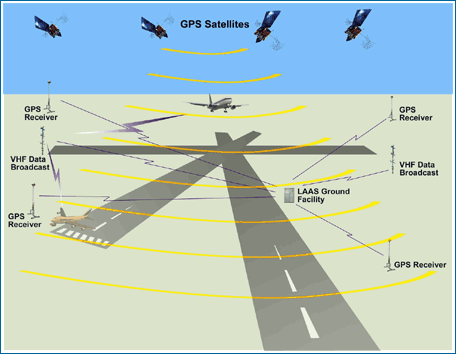
\includegraphics{figures/LAAS_Architecture.png}}
	}
	\caption{Local Area Augmentation System}
	\label{fig:FAA_LAAS}
\end{figure}







\section{\ac{gps} \& \ac{waas} Introduction}\label{gps-waas-introduction}

The are numerous navigation aids supporting the national airways. Many
are ground based but with the inception of \ac{gps} there is a transition to space based navigation. In regards to utilizing \ac{gps} and \ac{waas} for navigation there are questions that need to be answered as to the necessity of \ac{waas} and why \ac{gps} by itself is not sufficient for aircraft navigation.

\begin{itemize}
\tightlist
\item
  Why yet another navigation system?
\item
  What are the benefits over other ground based navigational aids?
  \begin{itemize}
  \tightlist
    \item
      \ac{ndb}
    \item
      \ac{dme}
    \item
      \ac{vor}
    \item
      \ac{ils}
  \end{itemize}
\item
  What is \ac{waas}?
\item
  Why can \ac{gps} not be used on its own?
\item
  What does \ac{waas} do?
\item
  How does \ac{waas} work?
\item
  Where is \ac{waas} used?
\item
  Why use \ac{gps} and \ac{waas}?
\end{itemize}

\subsection{\ac{faa} Air Transportation System
Modernization}\label{faa-air-transportation-system-modernization}

The \ac{faa} has recognized the need to improve the Air Transportation System
so that it is more efficient, more predictable, and able to handle more
capacity while maintaining the highest safety standards and reducing
environmental impacts. The \ac{faa}'s NextGen modernization initiative is
geared toward moving away from ground-based to satellite-enabled
technologies for navigation and surveillance systems and from analog to
digital systems for communication. While \ac{waas} is not a NextGen program,
it is one of the foundational pillars upon which satellite enabled
technologies are built.

\subsection{Benefits of the Wide Area Augmentation
System}\label{benefits-of-the-wide-area-augmentation-system}

\subsubsection{Primary Means of
Navigation}\label{primary-means-of-navigation}

\ac{waas} is a critical component of the modernization's effort to enable the
aviation industry's use of space-based navigational aids as a primary
means of navigation, including: takeoff, en-route, approach and landing.

\subsubsection{More Direct Routes}\label{more-direct-routes}

Space-based navigational aids allows more direct routes to be utilized
over ground based navigational aids. It is not restricted by location of
ground-based equipment or line of sight as with some ground base
equipment. For example, utilizing \ac{vor}, which is a ground-based
navigational aid, is equivalent to navigating along a highway in the
sky. Using a \ac{vor} network, aircraft fly from one \ac{vor} to another which may
not be the most direct path. Utilizing \ac{gps} and \ac{waas} aircraft can fly
direct routes from their departure point to arrival point.

\subsubsection{Approach with Vertical Guidance
Capability}\label{approach-with-vertical-guidance-capability}

Additionally \ac{waas} approaches with
vertical guidance capability can be utilized at many airports for
landing. The number of airports that utilize \ac{waas} approaches has now exceeded that of airports using the
\ac{ils} which is another ground-based aid for landing
aircraft. The advantage of using \ac{waas} approaches as opposed to
\ac{ils} approaches is that \ac{waas} approaches do
not require ground-based equipment at the destination runways. The
infrastructure for an \ac{ils} requires antenna
arrays at the far end of the runway along with middle and outer markers
located along an established line-of-sight route to a destination
runway. The middle marker is 3000 to 6000 feet from the runway and the
outer marker is 4 to 7 miles. This is just for a single runway end. If
aircraft need to land from the opposite runway end all of this equipment
is duplicated and mirrored. The \ac{ils} infrastructure can be costly and
problematic and a full complement of equipment must be installed for
each runway end. Adding to the cost, an \ac{ils} needs its antennas and
markers routinely calibrated. It is an expensive installation, serves
only one runway end and requires ongoing calibration for each
installation.

\href{https://en.wikipedia.org/wiki/Marker_beacon}{ILS Marker Beacon}
{[}Link: NextGen Frequently Asked Questions{]}{[}1{]}\\
{[}Link: Performance Success Stories New WAAS Coverage Clears the Way
for New Access to Airports{]}{[}2{]}

Another deficiency is that it can just land aircraft, but it cannot
provide guidance for departures, missed approaches or any other
navigational service. If a missed approach is required the \ac{ils} cannot aid the aircraft on its outbound route. With
\ac{waas} a missed approach route can be defined. This is useful in areas
like Kodiak Alaska where the approach leads directly into the base of
Barometer Mountain; if a missed approach is required the pilot has to
bank hard left between the valley created by Barometer Mountain and Old
Women's Mountain. With the \ac{ils} or other
ground-based navigational aids rugged or mountainous terrain can make
line-of-sight systems unachievable. Space based navigation can have
issues in areas like urban canyons, but for aviation applications, space
based navigation has few impediments.

\href{https://www.google.com/maps/@57.7483115,-152.5265434,13z/data=!4m3!11m2!2s1o5YgbCjAjyBntt5HWecW-6ByCvg!3e3!5m1!1e4}{Kodiak
Alask Map}

Another benefit of \ac{waas} is that the ground-based infrastructure does not
have to be expanded to expand the capabilities of \ac{waas}. More approaches
can be added by surveying the runway ends and approach vector utilizing
\ac{gps} waypoints. The application is separate from the infrastructure. Just
as in \ac{gps} for vehicle navigation; \ac{gps} is providing positioning and
timing services and the applications of those services are ever
expanding.

\subsubsection{Decommission of Older, Expensive Ground-Based Navigation
Equipment}\label{decommission-of-older-expensive-ground-based-navigation-equipment}

As satellite navigation systems become the primary means of navigation
and supplants those capabilities of older ground-based navigational aids
those aids can be decommissioned. As more approaches are defined more
\acp{ils} can be the decommissioned. As direct en-route capabilities are
established the \ac{ndb}, \ac{dme} and \ac{vor} systems can also be decommissioned.

\href{https://www.uasc.com/docs/default-source/documents/universalflyer/uasc_universalflyer_20122q.pdf?sfvrsn=e717985c_2}{FAA
Announces Plan for Reduction in VOR and ILS in Favor of WAAS}

\subsubsection{Simplified Avionics}\label{simplified-avionics}

With the implementation of \ac{waas} and \ac{laas}, as currently planned by the \ac{gps} Product Team, a substantial reduction in the user avionics equipment cost can be realized because of the reduction in the proliferation of navigational devices. A single device can serve all phases of flight.

\href{https://www.faa.gov/about/office_org/headquarters_offices/ato/service_units/techops/navservices/gnss/library/satnav/media/SatNavNews_Summer_2017.pdf}{The
Sum of All Performance-Based Navigation Procedures}

\subsubsection{Increased Capacity}\label{increased-capacity}

\ac{waas} enabled receivers provide a highly accurate \ac{gps} position solution,
so an aircraft's position is known to a higher fidelity than has
previously been available. This, along with other technologies being
pursued by the \ac{faa}, will offer opportunities to reduce separation
standards. This reduction will be an incremental process based on
analysis of the evolving capabilities. Potential reductions include
non-radar separations in en route airspace and terminal separations due
to smaller obstacle clearance areas and protected airspace. Reduced
separation standards will directly translate into increased system
capacity that can safely fly in a particular volume of airspace,
benefiting the aviation user community.

\href{https://www.faa.gov/about/office_org/headquarters_offices/ato/service_units/techops/navservices/gnss/library/satnav/media/SatNavNews_Spring2014_final_web.pdf}{WAAS
Benefits Driving Equipage}

\subsubsection{Resiliency}\label{resiliency}

\ac{waas} does require a ground-based equipment infrastructure, but that
infrastructure is highly resilient and redundant and \ac{waas} enabled
applications can be implemented with no need to expand \ac{waas}
ground-based equipment. It has a dual ring active/active network along
with active standby and backup equipment. If an outage happens with any
one piece of \ac{waas} equipment it can be placed in standby mode until such
time as it is appropriate to send maintenance personnel to work on it.
This is different from the \ac{ils} or \ac{vor}
systems, where if that ground-based navigational aid has a malfunction,
that service is rendered unavailable until the repairs are completed.
Depending on the criticality of the system, \ac{faa} maintainers may need to
be out in the field in adverse weather conditions to restore service.
Some equipment locations, like Kotzebue, Alaska, are inhospitable most
of the year, so it makes it very precarious for maintainers to get out
to those facilities to restore equipment and services. For \ac{waas}, a loss
of a subsystem does not mean a loss of service. Though it is not
optimal, with the redundancy build into \ac{waas} ground-based equipment
infrastructure it can run in a degraded state with no system impact
until conditions are suitable for the restoration.


\subsection{\ac{gps} Overview}\label{gps-overview}

\ac{waas} is a space-based differential \ac{gps} system. It is used to detect and correct \ac{gps} errors, monitor and correct for ionospheric delay and also
provides additional ranging sources from three GEO satellites for
improved availability of space based navigation services. It augments
\ac{gps} and improves accuracy, integrity, and availability. At its core \ac{waas} is a real-time \ac{gps} sensor network.


\subsection{Why can't you use \ac{gps} by
itself?}\label{why-cant-you-use-gps-by-itself}

\ac{waas} is an enhancement to \ac{gps} which monitors
and detects these associated errors and provides the necessary
corrections for meeting safety-of-life flight requirements. The purpose
of \ac{waas} is to monitor the \ac{gps} constellation and detect and correct for
errors when possible. If corrections are not possible \ac{waas} will alert
aviation users when \ac{gps} services cannot be used; the most notable being
ionospheric storm events where changes in the ionosphere are changing
too rapidly for the \ac{waas} ionoshperic model to adapt. \ac{waas} is able to
detect errors by utilizing a robust ground-based geographically diverse
sensor network. There are 38 \ac{waas} reference stations dispersed
throughout Alaska, Canada, continental US, Mexico and Hawaii. Each
reference station has three \ac{gps} receivers who's location coordinates are
precisely surveyed. Errors in the \ac{gps} signal can be detected and these
errors are grouped into two different classes; the \ac{udre} and the Grid Ionospheric Vertical Error. One is a per \ac{gps} satellite based correction and the other is a geographical based correction to account for the delay of the \ac{gps} signal through the ionosphere. How this works for the end user is that their avionics receiver calculates a protection level. If their protection level is within the alert limits specified in the \ac{waas} \ac{mops} then \ac{waas} services available for them and they can utilize \ac{waas} corrections to increase their accuracy. If however, they calculate a protection level that is outside the alert limit then \ac{waas} is unavailable for them and
they can not use the \ac{waas} service. There exist a case that a protection
level is calculated and it is within the alert limit but the true
position of the aircraft is outside of those boundaries. This is the
situation where the user determined they are safe when they are not.
This is called Hazardously Misleading Information (HMI). This is an area
in which National Airways System Engineering spends considerable time
evaluating to ensure users are protected.

\ac{waas} has mitigations and corrections for each type of error. First, \ac{waas}
mitigates the user clock error by using cesium atomic clocks. This is a
highly stable and accurate time source that disciplines the clock of the
\ac{gps} receiver used by the \ac{waas} reference station. It mitigates multipath
interference by using a highly specialized multipath limiting antenna.
\ac{waas} has an orbit determination filter to minimize the ephemeris errors
of \ac{gps} and GEO satellites. \ac{waas} also utilizes a Kriging model for the
ionosphere and provides ionospheric corrections for all of North
America. By mitigating the error sources in the acquisition of the \ac{gps}
measurement data, \ac{waas} is able to detect \ac{gps} errors and provide corrects
for those errors to users to increase their accuracy.

\subsection{What is \ac{waas}}\label{what-is-the-wide-area-augmentation-system-waas}

\ac{waas} is a space-based differential
\ac{gps} system. It detects and corrects \ac{gps} errors, monitors and corrects
for ionospheric delay and provides additional ranging sources for
improved availability of the navigational service. It augments \ac{gps} and
improves its accuracy, integrity and availability. At its core \ac{waas} is a real-time sensor network and the
sensor is a \ac{gps} antenna tracking all \ac{gps} satellites in view of that
antenna.

\subsection{What is the purpose of
\ac{waas}?}\label{what-is-the-purpose-of-waas}

\ac{waas} is designed to protect users from error sources and other threats
inherent in using \ac{gps}. It does this by broadcasting a \ac{udre}, a \ac{give} and \ac{gps}
health information to the user. \ac{waas} has predefined alert limits fixed
by specification. The aircraft's \ac{waas} enabled avionics will calculate
its \ac{gps} position while applying the \acp{wum} which have the
\ac{udre} and the \ac{give} values. The avionics receivers use these values to
calculate a protection level based on the algorithm specified in the
\ac{waas} \ac{mops}. If its protection level is within the alert limits then \ac{waas}
is available for that user. If it calculates the protection level and it
is beyond the alert limit then \ac{waas} is not available for that user. If
the protection level cylinder becomes too small and does not enclose the
true position of the aircraft this is called hazardously misleading
information. It is a scenario in which the calculated protection level
misinforms the user that the system is available for them to use when it
is not.

\subsection{How does \ac{waas} work?}\label{how-does-waas-work}

\subsubsection{\ac{wrs}}\label{waas-reference-stations}

The \ac{gps} satellites broadcast their ranging signal and message data down
to earth and it is collected at a 1Hz rate by a network of \ac{wrs}. There are 38 reference stations that are
geographically diverse across North and Central America including
Alaska, Canada, Continental US, Mexico and Hawaii. Each reference
station has three threads denoted as thread A, B and C, so 114
individual threads. The A and B threads of each reference station are
primarily utilized and the C thread is an active standby. A \ac{wrs} can
withstand an outage from any one thread. In fact \ac{waas} can withstand the
outage of one or more complete reference stations as long as they are
not in close geographical proximity to on another. If multiple reference
stations are out of service in a local area this will impact the
ionospheric model and coverage will be reduced or lost in that area. \ac{gps}
measurement data from every \ac{gps} satellites being tracked by all 114
threads is put onto a high availability terrestrial communications
network. The network connects the reference stations to the \ac{wms}.

\subsubsection{Wide-Area Master Station (WMS)}\label{waas-master-stations}

There are three \ac{wms} that pull in the \ac{wrs} data and
calculate the differential \ac{gps} corrections, ionospheric correction and
validates the \ac{gps} satellites are operating in a healthy normal mode. If
a satellite is not usable \ac{waas} will send a \ac{dnu} alert
message out to the users. These master stations are what calculate all
the integrity parameters and is the computational center point of the
system. The software for all the integrity monitors is running on a
real-time operating system and is maintained using the guidelines
specified in DO-178B, Software Considerations in Airborne Systems and
Equipment Certification up to a Software Level of B/Hazardous. Once all
the integrity parameters, the corrections and health information are
validated and calculated the information is formulated into a series of
\acp{wum} and then put on the terrestrial communications
network and sent to the \ac{gus}.

\subsubsection{GEO Uplink Subsystem}\label{geo-uplink-subsystem}

\ac{waas} has three GEO satellites. Each satellite has two uplink stations
denoted as primary and backup. The denotation for each system is based
on which station is radiating to the satellite. The \ac{gus}
that is radiating to the satellite is designated as primary and the
other, which is radiating into a dummy load, is denoted as backup. If
for some reason the primary has a failure it will automatically switch
to the backup and the backup will become primary. When the faulted GEO
Uplink Subsystem is restored to service it will be brought up into
backup mode. It will stay in backup mode until the primary faults and
automatically switches over back to primary or the \ac{waas} operator issues
a command to initiate a manual GUS switch over. This is done for
maintenance activities at GUS sites.

The \ac{gus} sends the \ac{wum} through the \ac{rfu} which broadcast it to the \ac{waas} satellite in
geosynchronous orbit. The \ac{waas} GEO satellite broadcasts the differential
and ionospheric corrections as well as \ac{gps} satellite heath back down to
the aviation users. The avionic equipment applies the \ac{waas} corrections
to increase the accuracy of its \ac{gps} position solution. \ac{waas} provides
another service called GEO Ranging. The three \ac{waas} GEO satellites
provide a ranging signal that functions like a \ac{gps} signal. These
additional ranging sources help fill in the usable satellite
constellation and also provides better satellite geometry. This
increases the availability of using space based navigation services
because the \ac{gps} constellation has now been augmented with three
additional satellites. If a \ac{gps} satellite is taken out of service the
three \ac{faa} GEO ranging satellites will help fill in the constellation.
The geometry of the satellite constellation has values associated with
it called the dilution of precision. The more dispersed the
constellation the better its dilution of precision. The more tightly
grouped the satellite constellation is the worse the dilution of
precision. The better dilution of precision value the better the
position solution will be.

{[}Link: Dilution of Precision{]}{[}5{]}

\subsubsection{Operation and Maintenance
System}\label{operation-and-maintenance-system}

The \ac{waas} system has two operation and maintenance systems located in
Warrenton, VA and the other in San Diego, CA. This is where the \ac{waas}
operators monitor and control the \ac{waas} system.

\subsection{Where is \ac{waas} used?}\label{where-is-waas-used}

\ac{waas} currently uses three geosynchronous satellites with a footprint
that covers the entire Western Hemisphere. Coverage over the northern
slope of Alaska is particularly valuable to the \ac{faa} due to Alaska having
many general aviation users that utilize \ac{waas}. As of May 24, 2018, there
are 3,909 \ac{waas} Localizer Performance
with Vertical guidance (LPV) approach procedures serving 1,900 airports.
1,138 of these airports are Non-\ac{ils} airports. Currently, there are also
661 Localizer Performance (LP) approach procedures in the U.S. serving
495 airports.

{[}Link: Satellite Navigation - GPS/WAAS Approaches{]}{[}6{]}

\begin{center}\rule{0.5\linewidth}{\linethickness}\end{center}

\section{Items to look into:}\label{items-to-look-into}

One significant improvement \ac{waas} provides is the elimination of
errors for hot and cold temperatures that previously affected baro type
vertical navigation systems. \ac{waas} equipped receivers will automatically
notify the pilot of the most accurate level of service provided for that
given receiver, signal, and approach.

One significant difference between satellite based navigation as opposed
to ground based is that distances: Are given Along Track Distance (ATD)
during the final approach segment.

One primary difference between an RNAV approach with \ac{gps} and \ac{waas} is at
the missed approach point \ac{gps} suspends while \ac{waas} sequences to the
missed approach procedure.

\begin{center}\rule{0.5\linewidth}{\linethickness}\end{center}

The \ac{faa} will seldom, if ever, install a new \ac{ils}, opting instead for PBN
landing procedures, which save money. Further costs saving are gained by
reducing the existing ground-based navigation infrastructure, which
remains as a backup in case of disrupted satellite service. {[}1{]}:
https://www.faa.gov/nextgen/faqs/ {[}2{]}:
https://www.faa.gov/nextgen/snapshots/stories/?slide=5 {[}3{]}:
http://www.trimble.com/gps\_tutorial/howgps-timing2.aspx {[}4{]}:
https://gis.stackexchange.com/questions/40660/trilateration-algorithm-for-n-amount-of-points/40678\#40678
{[}5{]}:
https://en.wikipedia.org/wiki/Dilution\_of\_precision\_(navigation)
{[}6{]}:
https://www.faa.gov/about/office\_org/headquarters\_offices/ato/service\_units/techops/navservices/gnss/approaches/

https://www.faa.gov/about/office\_org/headquarters\_offices/ato/service\_units/techops/navservices/gnss/faq/gps/?iframe=true\&width=100\%\&height=100\%
Q. Is the basic \ac{gps} signal sufficient to meet all the needs of civil aviation?

A. This is not a simple yes/no answer. The answer is that it depends on
the service requirements of each user or aviation authority. For many
countries, \ac{gps} supplies a better capability than the existing
ground-based systems or lack thereof. Yet for other countries with large
infrastructures, the \ac{gps} signal does not meet the accuracy, integrity,
availability, and continuity requirements critical to safety of flight.
Enhancements to the \ac{gps} such as \ac{waas} and \ac{gbas} provide the necessary corrections for meeting safety-of-life flight requirements.

\begin{sidewaystable}[htbp]
\centering
\caption{\ac{waas} Sites}
\resizebox{\columnwidth}{!}{
\begin{tabular}{ l l l l l}
\hline
\textbf{City} &
\textbf{ICAO airport code} &
\textbf{Antenna 1} &
\textbf{Antenna 2} &
\textbf{Antenna 3}\\ \hline
Bethel, Alaska                           & PABE     & 60.787916486°N 161.841724416°W, 52.203 m    & 60.787897064°N 161.841663857°W, 52.204 m    & 60.787881127°N 161.841728605°W, 52.198 m\\
Billings, Montana                        & KBIL     & 45.803707088°N 108.539722283°W, 1112.261 m  & 45.803716383°N 108.539780649°W, 1112.266 m  & 45.803756811°N 108.539680968°W, 1112.255 m\\
Barrow, Alaska                           & PABR     & 71.282765883°N 156.789923397°W, 15.577 m    & 71.282798595°N 156.789965306°W, 15.589 m    & 71.282793925°N 156.789856228°W, 15.577 m\\
Cold Bay, Alaska                         & PACD     & 55.200334771°N 162.718472052°W, 53.648 m    & 55.200394330°N 162.718489390°W, 53.652 m    & 55.200400493°N 162.718623936°W, 53.657 m\\
Fairbanks, Alaska                        & PAFA     & 64.809630987°N 147.847339789°W, 149.891 m   & 64.809681435°N 147.847491409°W, 149.897 m   & 64.809748030°N 147.847379206°W, 149.876 m\\
Honolulu, Hawaii                         & PHNL     & 21.312988930°N 157.920824884°W, 24.678 m    & 21.312645960°N 157.920980760°W, 25.022 m    & 21.312714586°N 157.920825156°W, 25.067 m\\
Juneau, Alaska                           & PAJN     & 58.362575024°N 134.585705943°W, 16.024 m    & 58.362469451°N 134.585487326°W, 16.029 m    & 58.362545895°N 134.585292259°W, 16.020 m\\
Mérida, Yucatán                          & MMMD     & 20.931909130°N 089.662840352°W, 29.133 m    & 20.931901399°N 089.662887739°W, 29.171 m    & 20.931946482°N 089.662890840°W, 29.168 m\\
Mexico City                              & MMMX     & 19.431653203°N 099.068389471°W, 2236.638 m  & 19.431676477°N 099.068348099°W, 2236.625 m  & 19.431629899°N 099.068430820°W, 2236.652 m\\
Puerto Vallarta, Jalisco                 & MMPR     & 20.679003359°N 105.249202871°W, 10.973 m    & 20.679041461°N 105.249177972°W, 11.269 m    & 20.679059454°N 105.249221363°W, 10.990 m\\
San José del Cabo, Baja California Sur   & MMSD     & 23.160445938°N 109.717646195°W, 104.297 m   & 23.160383141°N 109.717652895°W, 104.285 m   & 23.160419201°N 109.717704568°W, 104.277 m\\
Tapachula, Chiapas                       & MMTP     & 14.791366074°N 092.367999089°W, 54.962 m    & 14.791334042°N 092.367965119°W, 54.950 m    & 14.791319966°N 092.368009440°W, 54.855 m\\
Kotzebue, Alaska                         & PAOT     & 66.887333160°N 162.611372024°W, 10.911 m    & 66.887368005°N 162.611390215°W, 10.909 m    & 66.887356742°N 162.611304386°W, 10.913 m\\
Iqaluit, Nunavut                         & CYFB     & 63.731490169°N 068.543181586°W, 10.022 m    & 63.731464001°N 068.543402553°W, 9.957 m     & 63.731386362°N 068.543596671°W, 10.014 m\\
Gander, Newfoundland and Labrador        & CYQX     & 48.966489496°N 054.597631164°W, 146.888 m   & 48.966447606°N 054.597532034°W, 146.887 m   & 48.966406383°N 054.597433025°W, 146.899 m\\
Winnipeg, Manitoba                       & CYWG     & 49.900574663°N 097.259396222°W, 222.042 m   & 49.900677586°N 097.259217224°W, 222.051 m   & 49.900568446°N 097.259226893°W, 222.045 m\\
Goose Bay, Newfoundland and Labrador     & CYYR     & 53.308646665°N 060.419467188°W, 37.830 m    & 53.308713007°N 060.419365697°W, 37.844 m    & 53.308803193°N 060.419371104°W, 37.853 m\\
Albuquerque, New Mexico                  & KZAB     & 35.173575457°N 106.567349162°W, 1620.117 m  & 35.173574799°N 106.567287780°W, 1620.181 m  & 35.173532365°N 106.567287878°W, 1620.164 m\\
Anchorage, Alaska                        & PAZA     & 61.229202467°N 149.780248917°W, 80.660 m    & 61.229118812°N 149.780422686°W, 80.653 m    & 61.229202391°N 149.780423003°W, 80.648 m\\
Aurora, Illinois                         & KZAU     & 41.782657876°N 088.331335953°W, 195.918 m   & 41.782595526°N 088.331334442°W, 195.921 m   & 41.782596464°N 088.331253756°W, 195.926 m\\
Nashua, New Hampshire                    & KZBW     & 42.735720140°N 071.480425027°W, 39.125 m    & 42.735724128°N 071.480358015°W, 39.151 m    & 42.735671312°N 071.480352294°W, 39.147 m\\
Leesburg, Virginia                       & KZDC     & 39.101595603°N 077.542745736°W, 80.084 m    & 39.101523590°N 077.542730286°W, 80.080 m    & 39.101548982°N 077.542774296°W, 80.092 m\\
Longmont, Colorado                       & KZDV     & 40.187303318°N 105.127223496°W, 1541.399 m  & 40.187303552°N 105.127154188°W, 1541.391 m  & 40.187253096°N 105.127167214°W, 1541.377 m\\
Fort Worth, Texas                        & KZFW     & 32.830649739°N 097.066471191°W, 155.617 m   & 32.830596303°N 097.066523654°W, 155.576 m   & 32.830598335°N 097.066470282°W, 155.620 m\\
Houston, Texas                           & KZHU     & 29.961896297°N 095.331425748°W, 10.908 m    & 29.961831785°N 095.331449752°W, 10.974 m    & 29.961773563°N 095.331512004°W, 10.958 m\\
Hilliard, Florida                        & KZJX     & 30.698859379°N 081.908184568°W, 2.149 m     & 30.698823791°N 081.908152480°W, 2.140 m     & 30.698791217°N 081.908198025°W, 2.135 m\\
Olathe, Kansas                           & KZKC     & 38.880159315°N 094.790833106°W, 305.904 m   & 38.880160009°N 094.790643592°W, 305.903 m   & 38.880101810°N 094.790710614°W, 305.636 m\\
Palmdale, California                     & KZLA     & 34.603517830°N 118.083893947°W, 763.521 m   & 34.603517881°N 118.083828796°W, 763.520 m   & 34.603473855°N 118.083893956°W, 763.598 m\\
Salt Lake City, Utah                     & KZLC     & 40.786043564°N 111.952176782°W, 1287.421 m  & 40.785990178°N 111.952176149°W, 1287.416 m  & 40.785990067°N 111.952122320°W, 1287.423 m\\
Miami, Florida                           & KZMA     & 25.824611968°N 080.319189364°W, -7.579 m    & 25.824659706°N 080.319315758°W, -8.207 m    & 25.824661752°N 080.319234381°W, -7.861 m\\
Memphis, Tennessee                       & KZME     & 35.067394005°N 089.955369299°W, 68.609 m    & 35.067437537°N 089.955368937°W, 68.883 m    & 35.067439374°N 089.955436864°W, 68.871 m\\
Farmington, Minnesota                    & KZMP     & 44.637463181°N 093.152084552°W, 262.679 m   & 44.637463059°N 093.152011267°W, 262.693 m   & 44.637407004°N 093.152022108°W, 262.628 m\\
Ronkonkoma, New York                     & KZNY     & 40.784328238°N 073.097164869°W, 6.457 m     & 40.784275495°N 073.097154931°W, 5.930 m     & 40.784275925°N 073.097223653°W, 5.936 m\\
Fremont, California                      & KZOA     & 37.543053122°N 122.015945899°W, -3.497 m    & 37.543025498°N 122.015892540°W, -3.481 m    & 37.542981164°N 122.015929270°W, -3.400 m\\
Oberlin, Ohio                            & KZOB     & 41.297154278°N 082.206443927°W, 223.689 m   & 41.297166589°N 082.206351733°W, 225.187 m   & 41.297086827°N 082.206379312°W, 223.468 m\\
Auburn, Washington                       & KZSE     & 47.286993478°N 122.188372098°W, 82.112 m    & 47.286907917°N 122.188382169°W, 82.168 m    & 47.286856213°N 122.188363949°W, 82.105 m\\
San Juan, Puerto Rico                    & TJZS     & 18.431335686°N 065.993476761°W, -28.062 m   & 18.431218583°N 065.993514086°W, -28.047 m   & 18.431198889°N 065.993448100°W, -28.108 m\\
Hampton, Georgia                         & KZTL     & 33.379688402°N 084.296725378°W, 261.138 m   & 33.379691546°N 084.296656313°W, 261.126 m   & 33.379634831°N 084.296652682°W, 261.161 m\\
\end{tabular}
}
\label{tab:WAAS_SITES}
\end{sidewaystable}




\ac{laas} was initiated by the \ac{faa} to provide an accurate real time differential \ac{gps} solution . The \ac{laas} concept follows that of \ac{waas}, but the reference receivers are generally located within the airport environment as can be seen in Figure~\ref{fig:FAA_LAAS}.  Further, the differential \ac{gps} corrections are only usable within the VDB broadcast range, which is about 20 to 30 miles.  By limiting the operating region \ac{laas} is able to deliver accuracy under 1 meter in both the horizontal and vertical axis\cite[]{FAA_LAAS}. A further benefit is that \ac{laas} is only dependent on the \ac{gps} fleet; therefore it can be used anywhere in the world.  The \ac{faa} formalized the interfaces and many of the algorithms that should be used in a \ac{lgf}. Components of a software architecture for a \ac{laas} will be examined in the remainder of this dissertation, including the host architecture, message formats, and message broadcasting.

\newpage

\newpage
\thispagestyle{empty}
\chapter{Methodology}
\label{ch:methodology}
\section{Solution Stack}
Reproducibility is one of the main principles of the scientific method and within the \ac{faa} having tools and processes that can reliably reproduce results is paramount for a safety of life application.  In this section the solution stack will be introduced. And from the ground up the applications selected and process implemented are to ensure results can be reproduced by those that have access to the data store.

A solution stack or software stack is a set of software subsystems or components needed to create a complete platform such that no additional software is needed to support applications. Applications are said to "run on" or "run on top of" the resulting platform.

This section covers the following components of the solution stack: virtualization platform, operating system, orchestration, web server, databases, programming language and analytics environment. Further effort is required for a few remaining components of the final solution stack, mostly needed for scaling. The remaining components are orchestration, job scheduling, workload management and horizontal scaling.

\subsection{Virtualization}
Server scaling can come in two varieties: horizontal and vertical.  Horizontal scaling is adding more server nodes to an application to handle the additional workload demand, while vertical scaling or scaling up is to add more resources to one node.  This solution stack uses virtual machines to scale horizontally; to handle an increase in workload, as well as provide high availability, additional virtual machines can be provisioned and when the demand subsides the virtual machines can be deallocated.  The use of virtual machines can streamline development since they can repeatedly be created and destroyed to test out configurations.

\subsubsection{Vagrant with VirtualBox Provider}
The first component of the solution stack is \emph{Vagrant}. Its primary use is to create and configure virtual development environments.  It also helps manage those virtual environments with a few very simple commands. The advantage of using this product is that is can be used by anyone on any platform that Vagrant supports to bring up an identical working environment. Through a Vagrant configuration file it can even constrain the virtual image to a specific version or versions of a image. It also has the capability to automatically install all the additional required applications in the solution stack so that when the system boots up the first time all required software has been installed and configurations have been completed.

This solution stack currently uses Oracle VirtualBox, but it is compatible with other virtualization software like VMware and KVM. The final virtual machines will run on VMWare in a blade cluster.

\subsubsection{Vagrant Lifecycle Management}

\paragraph{Command: {\color{red} vagrant init [box-name] [box-url]}} ~\\
By default Vagrant will use the containing directory of the Vagrant initialization file, called Vagrantfile, for the virtual machine name. To get started with Vagrant, first create a new directory and change into that directory.
\begin{lstlisting}
mkdir WAASAnalyticsPlatform && cd WAASAnalyticsPlatform
\end{lstlisting}

The following commands initialize the current directory to be a Vagrant environment by creating the initial Vagrantfile. The Vagrant virtual image is known as a box. If a first argument is given, it configure the Vagrantfile for that type of box.

\begin{lstlisting}
# Example: Create an Ubuntu 14.04 virtual machine.
vagrant init ubuntu/trusty64
# Example: Create a CoreOS virtual machine.
# Exit the WAASAnalyticsPlatform folder
cd ..
# Checkout a CoreOS Vagrantfile from github.
git clone https://github.com/coreos/coreos-vagrant/
# This will create a coreos-vagrant directory in the
# current directory. Rename this directory to the name
# that the virtual machine will be known as.
mv coreos-vagrant CoreOS-Node01
\end{lstlisting}

\paragraph{Note: Unless otherwise stated the following commands must be ran in the folder containing the Vagrantfile and the command will apply to that environment.}

\paragraph{Command: {\color{red} vagrant up}} ~\\
This command creates and configures guest machines according to your Vagrantfile.

This is the single most important command in Vagrant, since it is how any Vagrant machine is created. Anyone using Vagrant must use this command on a day-to-day basis.

\paragraph{Command: {\color{red} vagrant halt}} ~\\
This command shuts down the running machine Vagrant is managing.

Vagrant will first attempt to gracefully shut down the machine by running the guest OS shutdown mechanism. If this fails, or if the -{}-force flag is specified, Vagrant will effectively just shut off power to the machine.

\paragraph{Command: {\color{red} vagrant ssh}} ~\\
This will SSH into a running Vagrant machine and give you access to a shell.

If a -{}- (two hyphens) are found on the command line, any arguments after this are passed directly into the ssh executable. This allows you to pass any arbitrary commands to do things such as reverse tunneling down into the ssh program.

\paragraph{Command: {\color{red} vagrant status}} ~\\
This will tell you the state of the machines Vagrant is managing.

It is quite easy, especially once you get comfortable with Vagrant, to forget whether your Vagrant machine is running, suspended, not created, etc. This command tells you the state of the underlying guest machine.

\paragraph{Command: {\color{red} vagrant destroy}} ~\\
This command stops the running machine Vagrant is managing and destroys all resources that were created during the machine creation process. After running this command, your computer should be left at a clean state, as if you never created the guest machine in the first place.

\paragraph{Command: {\color{red} vagrant global-status} and Using IDs} ~\\

To interact with any of the machines, you can go to
the directory with the Vagrantfile and run any of the preceding vagrant commands. Vagrant also provides a way to interact with the virtual machines without having to change into the directory. The global-status is the command that lists information and status about all known Vagrant environments
on the host machine.  The first column is the ID for the machine and the preceding commands all take an ID as an ending argument.
\lstset{basicstyle=\tiny}
\begin{lstlisting}[language=bash]
vagrant global-status
id       name    provider   state    directory
------------------------------------------------------------------------------------------------
26d0e63  default virtualbox poweroff /home/csherrell/Vagrant/v-Ubuntu-14.04-Bootstrap
d6e2bc0  default virtualbox poweroff /home/csherrell/Vagrant/v-Ubuntu-14.04-Rabbit-02
fc44416  default virtualbox poweroff /home/csherrell/Vagrant/v-Ubuntu-14.04-Rabbit-01
77c195d  default virtualbox poweroff /home/csherrell/Vagrant/v-Ubuntu-14.04-Rabbit-Cassandra-01
\end{lstlisting}


This shows that all the virtual machines are off. To start the first virtual machines run the following command.

\begin{lstlisting}[language=bash]
vagrant up 26d0e63
...
vagrant global-status
id       name    provider   state    directory
------------------------------------------------------------------------------------------------
26d0e63  default virtualbox running  /home/csherrell/Vagrant/v-Ubuntu-14.04-Bootstrap
d6e2bc0  default virtualbox poweroff /home/csherrell/Vagrant/v-Ubuntu-14.04-Rabbit-02
fc44416  default virtualbox poweroff /home/csherrell/Vagrant/v-Ubuntu-14.04-Rabbit-01
77c195d  default virtualbox poweroff /home/csherrell/Vagrant/v-Ubuntu-14.04-Rabbit-Cassandra-01
\end{lstlisting}

To start the remaining virutal machines run the following command.
\begin{lstlisting}[language=bash]
vagrant up d6e2bc0 fc44416 77c195d
...
vagrant global-status
id       name    provider   state   directory
-----------------------------------------------------------------------------------------------
26d0e63  default virtualbox running /home/csherrell/Vagrant/v-Ubuntu-14.04-Bootstrap
d6e2bc0  default virtualbox running /home/csherrell/Vagrant/v-Ubuntu-14.04-Rabbit-02
fc44416  default virtualbox running /home/csherrell/Vagrant/v-Ubuntu-14.04-Rabbit-01
77c195d  default virtualbox running /home/csherrell/Vagrant/v-Ubuntu-14.04-Rabbit-Cassandra-01
\end{lstlisting}

\lstset{basicstyle=\normalfont}

\noindent
Vagrant Website:~\\
\url{https://www.vagrantup.com/}

\subsection{Software Development}
\subsubsection{Python 3}
Python version 3 is being used for this development effort. The Python programming language guidance is ``if you can do exactly what you want with Python 3.x" then you should use it. During a previous phase of development a NovAtel binary message parser was written in Python 2.7 to parse log messages. This plus some other support software written in Python 2.7 was converted to version 3. The new parsing code is completely object oriented and the new classes for handling NovAtel messages where all written in Python 3 and there were no major issues.  The only issue that has reoccurred was in integrating the message parsing functionality developed in Python 2.7 into the new classes. Python 3 strings are Unicode by default and now there is clean Unicode/bytes separation.  For the average use case this has little to no affect, but when the purpose of the application is to read in a binary data stream and manipulate bytes this has a significant impact.  In Python 2.7 strings and bytearray objects could be use interchangeably. Under Python 3 this is no longer the case. Python 3 will throw a run time exception if a string is cast to a bytearray or vica versa. In Python 3 to convert bytes or bytearray objects to ASCII strings the decode method must be called.

\lstset{basicstyle=\tiny}
\begin{lstlisting}[language=Python]
# Hello World! in Hex
input_buffer = bytearray.fromhex('48656c6c6f20576f726c6421')
ascii_string = 'Test: '
# Append the bytearray to the string
ascii_string += input_buffer[0:]
\end{lstlisting}
\begin{lstlisting}[language=bash]
---------------------------------------------------------------------------
TypeError                                 Traceback (most recent call last)
<ipython-input-17-f84d039df76b> in <module>()
----> 1 ascii_string += input_buffer[0:]

TypeError: Can't convert 'bytearray' object to str implicitly
\end{lstlisting}
\begin{lstlisting}[language=Python]
# Using the bytearray.decode() method
ascii_string += input_buffer[0:].decode('ascii')
print(ascii_string)
Test: Hello World!
\end{lstlisting}
\lstset{basicstyle=\normalfont}

This analysis platform uses a producer/consumer architecture. To publish data to a queuing middleware used by the downstream consumers the data must first be serialized. Serialization is the conversion of data structures to a steam of bits to be saved to disk or transported across a communication medium. Under Python 2.7 there is a built-in Python module called pickle that is used for serialization but it was not well optimized, so the msgpack module was use for initial testing. As more involved testing was performed it was discovered that the msgpack module could not serialize all the data elements.  Luckily this happened about the same time as the transition to Python 3.  The msgpack module has deficiencies and further it has not yet been ported to Python 3.  Under Python 2.7 there was an optimized C implementation of the pickle module and under Python 3 the built-in pickle module is the C optimized implementation, so msgpack was dropped all together and pickle was used as the serialization service throughout the software.

\noindent
\\Python Website:\\
\url{https://www.python.org}\\
\url{https://wiki.python.org/moin/Python2orPython3}

\subsubsection{Messaging / Middleware}
Middleware is the software that connects software components or enterprise applications. Middleware is the software layer that lies between the operating system and the applications on each side of a distributed computer network. Typically, it supports complex, distributed business software applications.

This analysis platform uses a distributed producer consumer architecture.  Currently this is built upon the RabbitMQ middleware, but the decoupled software architecture will allow for one middleware to be swapped for another or have the ability to use multiple at once. ZeroMQ is another middleware that will be evaluated in the future as other entities in the FAA use it.
\paragraph{RabbitMQ} ~\\
RabbitMQ is an implementation of the \ac{amqp}. \ac{amqp} was designed by JPMorgan Chase and is used extensively in the financial industry.  Multiple implementation of \ac{amqp} have been created, but RabbitMQ is one of the more prestigious implementation. It is used throughout the VMware product line and also used in OpenStack for messaging. It supports several different type of exchanges: Direct, Fanout, Topic, and Headers; and can support persistent queues. The Python library that supports the interaction with RabbitMQ service is called Pika and will be covered later.

\paragraph{ZeroMQ} ~\\
ZeroMQ is a high-performance asynchronous messaging library, aimed at use in distributed or concurrent applications. It provides a message queue, but unlike message-oriented middleware, like RabbitMQ, ZeroMQ can run without a dedicated message broker. This product will be evaluated in the future and could augment the messaging capabilities in this application. The \ac{sog} in the \ac{faa} use ZeroMQ so some functionality may be required to be able to store and access data in their database.

\subsection{Databases and Storage Formats}
Several databases and storage formats have already been and will be evaluated during this research effort.  Databases serve a couple of different purposes. First and foremost they store and retrieve data.  The advantage a database has over comma separated \ac{ascii} files is that the data comes in as binary and is stored as binary there by avoiding precision being lost when floating point values are converted to \ac{ascii}.  Another advantage is that databases are useful for performing data analysis.  In the past databases were used primarily to do \ac{oltp}, basically data entry and retrieval transaction processing and run some standard reports. Today new databases support \ac{olap} which provides the capability for complex calculations, trend analysis, and sophisticated data modeling. This application like many modern applications will use polyglot persistence that is to say it will use the best persistence mechanism for the application's needs and that will probably utilize multiple types of storage engines. Beyond the ability to store and analyze data is the requirement to share data. Doing an analysis is one thing, but due to the integrity requirements of a safety of life system other organizations will be evaluating the results, so the input data, final solution and possibly some intermediate values should be save in such a way as to be able to hand over for independent evaluation.

\paragraph{Graphite's Whisper Database} ~\\
Whisper is a file-based time-series database format for Graphite. Graphite is a web analytics application for time-series data. The upside is that it has good community support and designed specificity for time-series data which is the bulk of the data being used in this research. The downside is that it only support one second resolution. This is acceptable for all the ac{waas} data that will initially be evaluated. A more advanced time series database may need to be assessed as additional sensors are incorporated that operate faster than 1Hz. Some of the temperature sensors and accelerometers that are currently being evaluated operate at 50Hz.

\noindent
\\Graphite Website:\\
\url{http://graphite.readthedocs.org/en/latest/}\\
\url{https://github.com/graphite-project/whisper}

{\Huge{{\color{red}{~\\Proofread Completed}}}}

\paragraph{PostgreSQL} ~\\
PostgreSQL is a relational database.  Relational databases are probably the most widespread of all database types, but their problem is that they are normally ran on one server and do not scale horizontally, but vertically. Typically this leads to a single point of failure, but there are some system administration paradigms that can support high availability. Also, there is significant overhead for indexing large datasets.  Because of there use in data warehousing many of these issues do have solutions or workarounds. Relational databases have been the standard for well over 40 years, so they have there place.  This application stack will use a relations database to store small datasets and will be used extensively to development models.

\paragraph{SQLite} ~\\
SQLite is an in-process library that implements a self-contained, serverless, zero-configuration, transactional relational database engine. The code for SQLite is in the public domain and is thus free for use for any purpose, commercial or private. SQLite is the most widely deployed database in the world. The data is contained in a single file so this would be a solution for sharing data amongst the various people wanting to use the data.

\paragraph{HDF5} ~\\
\ac{hdf} version 5 is not a database but a unique technology suite that makes possible the management of extremely large and complex data collections. The HDF5 technology suite includes: A versatile data model that can represent very complex data objects and a wide variety of metadata. The data is structured and remains in a binary format.  Matlab uses this a the base format for its MAT-File starting in R2006b. This file format is designed for very large datasets and since the dataset will be contained in one file it is being strongly considered as the format for sharing data with other organizations.

\paragraph{Cassandra} ~\\
Cassandra is a distributed database produces by Apache designed to handle large amounts of data across many server nodes. It is a big data database.


\iffalse
\subsection{Analytics}
\subsection{Application Program Interface}
\subsection{Apache Spark}


\subsubsection{Libraries}
\paragraph{Python Pika} ~\\
\paragraph{Python Sphinx} ~\\
\paragraph{Python HDF5} ~\\

\subsubsection{Orchestration}
\subsubsection{Jenkins}
\subsubsection{Juju/Puppet/Chef}
\subsubsection{Docker}

\section{Implementation}
\subsection{Versioning}
A version number is associated with each component of this software stack. Some of the software is \ac{cots} while other software has been custon written for this effort.

\begin{itemize}
	\item Operating System
	\item \ac{cots}
	\begin{itemize}
		\item MATLAB
	\end{itemize}
	\item Libraries
	\begin{itemize}
		\item Pika
	\end{itemize}
	\item Databases
	\begin{itemize}
		\item SQLite
		\item PostgreSQL
		\item Cassandra
	\end{itemize}
	\item Applications
	\begin{itemize}
		\item RabbitMQ
		\item Graphite
	\end{itemize}
\end{itemize}

\fi

\newpage

\newpage
\thispagestyle{empty}
\chapter{Results and Discussion}
\label{ch:results}
Currently the graphite database contains 1213 data element. In the plot below each data element is the leaf in the directory tree represented by a file icon. This plot for one the psuedorange and standard deviation from the \ac{gps} receiver. Each data element contains a data point for each second of the day, 86400 points.  This is just a first cut at getting data loaded into the system, but the design will support many data elements and calculations done between elements.
\\ \\
\resizebox{\columnwidth}{!}{
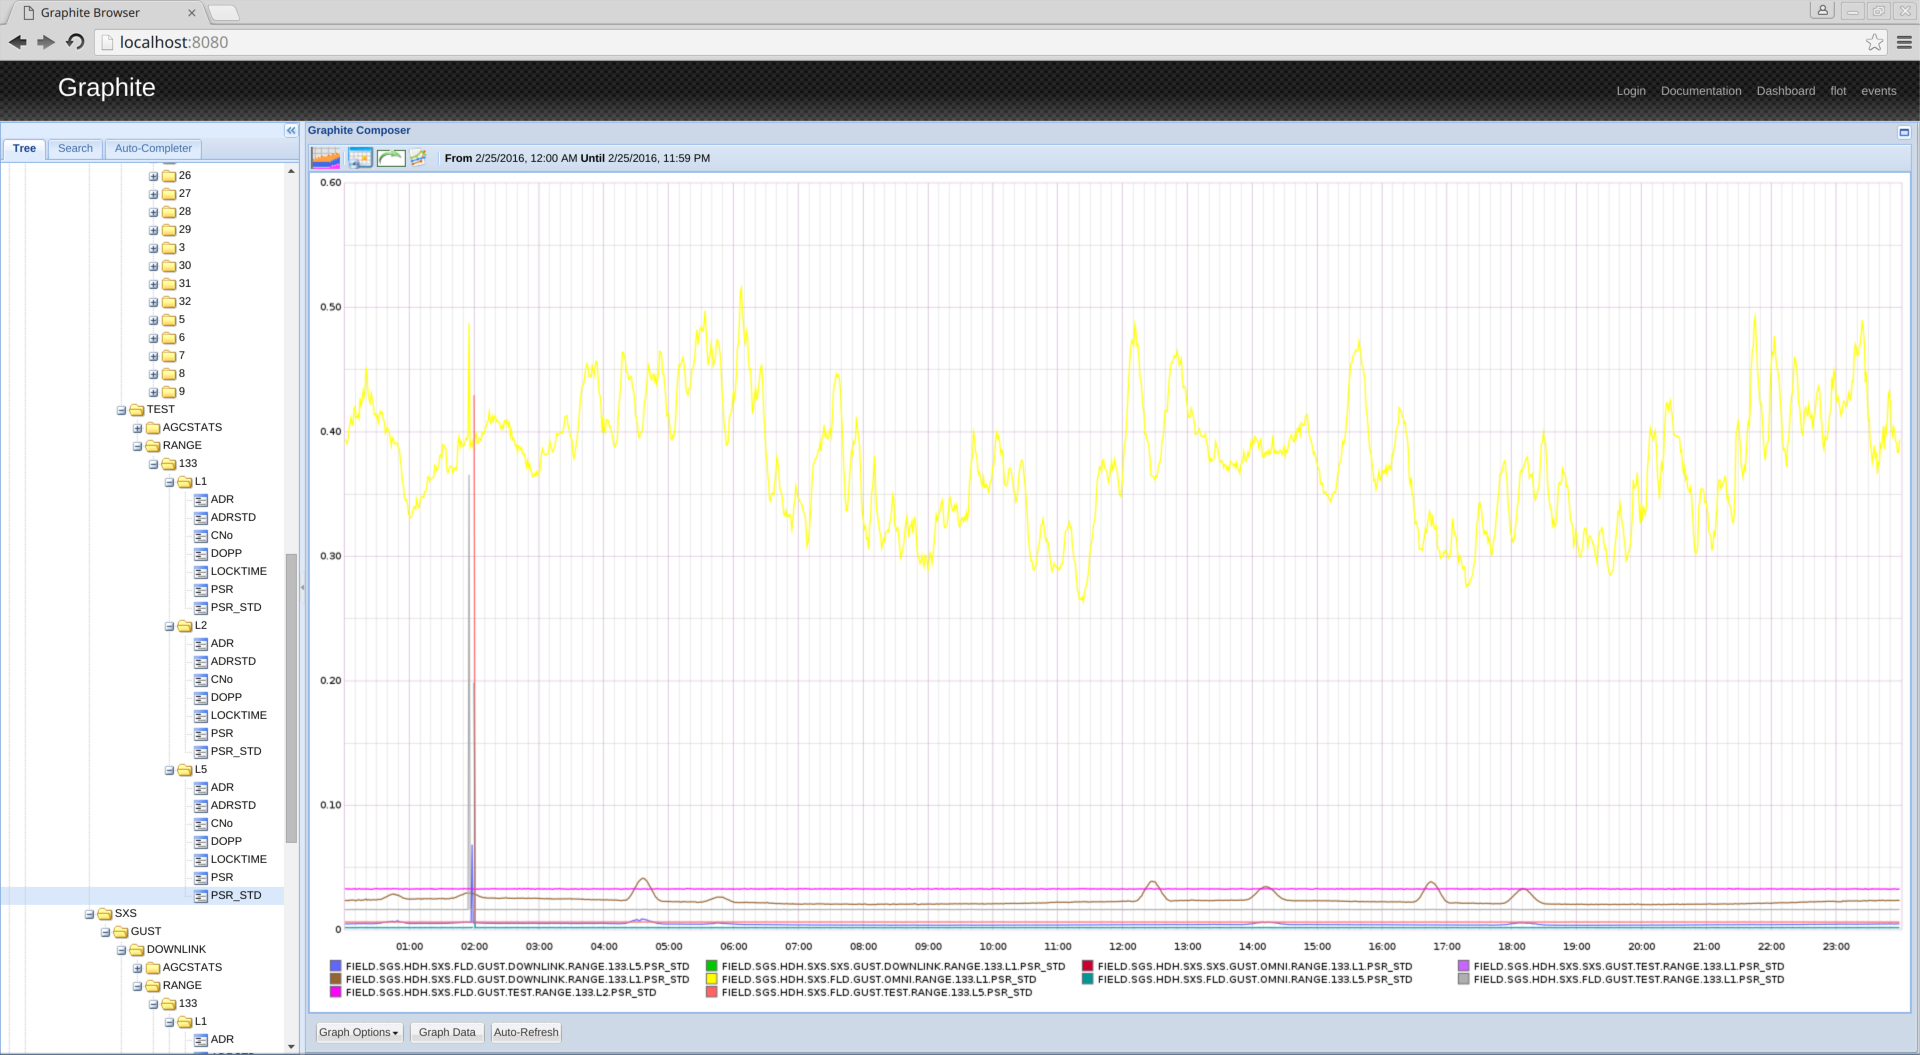
\includegraphics[scale=.25]{figures/PSR_STD-2016-02-25}
}

\newpage

\newpage
\thispagestyle{empty}
\chapter{Summary and Conclusions}
\label{ch:conclusions}
There is still a lot I need to get done, but progress is going well.  Currently I am having to interleave this into an already overloaded work schedule.  I am hoping to take some time off to devote to more writing.  I have more done that I have written here, but I just have not had a opportunity to write everything up.

Ideas for future research.

\newpage

% The University of Oklahoma (OU) requires single spacing for the bibliography
\singlespacing

% Style
%\bibliographystyle{IEEEtranS}
%% Bibliography or References - Required
%% Bibliography may contain multiple Bibtex files
%\bibliography{LiteratureReview,References}
\bibliographystyle{abbrv}
\bibliography{References}

\doublespacing % restore double spacing for the appendices

% Appendices - Optional
%\appendix   %if only one appendix chapter
\appendices % for multiple appendix chapters

\newpage
\thispagestyle{empty}
\chapter{DO-178B\label{chapter:DO-178B}}
The software levels as defined by DO-178B are:
\begin{description}
\item[Level A] Software whose anomalous behavior, as shown by the system safety assessment process, would cause or contribute to a failure of system function resulting in a catastrophic failure condition for the aircraft.

\item[Level B] Software whose anomalous behaviors, as shown by the system safety assessment process would cause or contribute to a failure of system function resulting in a hazardous/severe-major failure condition for the aircraft.

\item[Level C] Software whose anomalous behavior, as shown by the system safety assessment process, would cause or contribute to a failure of system function resulting in a major failure condition for the aircraft.

\item[Level D] Software whose anomalous behavior, as shown by the system safety assessment process, would cause or contribute to a failure of system function resulting in a minor failure condition for the aircraft.

\item[Level E] Software whose anomalous behavior, as shown by the system safety assessment process, would cause or contribute to a failure of system function with no effect on aircraft operational capability or pilot workload. 
\end{description}

\newpage
\thispagestyle{empty}
\chapter{Glossary}
\begin{description}
	\item[Reference Receiver (RR)] A Reference Receiver is composed of a Helibowl, Dipole, 2 GG12s, and 2 FreeWave Modems. 
	\item[LAAS Ground Facility (LGF)] The LAAS Ground Facility is the facility that equipment needed for LAAS.
	\item[LAAS Processing Unit (LPU)] The computing platform and software used to produce the LAAS SIS.
	\item[Local Area Augmentation System (LAAS)] LAAS designates all the components of this particular GBAS system.  It includes the Reference Receiver, LAAS Ground Facility, and any other infrastructure requirements.  
\end{description}

\end{document}
